\section{Advanced Topics in Deep Learning for Computer Vision}

\subsection{Recall on CNNs}

In representation learning we try to find good ways of representing data, often by learning a useful transformation of the raw data.
Deep learning is a subset of representation learning.

\subsubsection{Gradient descent}
Neural networks are usually trained using iterative, gradient-based optimizers that drive the cost function to a very low value.
The convergence point of gradient descent depends on the initial values of the parameters.
For feedforward neural networks it's important to initialize all weights to small random values and to initialize biases to zero or to small positive values.
To apply gradient based learning we must choose a cost function and how to represent the output of the model.
The derivative $f'(x)$ gives the slope of $f(x)$ at the point $x$.
The derivative is useful for minimizing a function because it tells us how to change $x$ in order to make a small improvement in $y$.
A point that obtains the absolute lowest value of $f(x)$ is a global minimum.

To reach the minimum we use the formula $w' = w - \alpha \frac{\partial J(w,b)}{\partial w} \,\, b' = b - \alpha \frac{\partial J(w,b)}{\partial b}$, where $\alpha$ is the learning rate, which controls how big are the steps that we take during the gradient descent.
If the slope is positive, we subtract the quantity in order to reach the minimum, or else we do the opposite thing.

As the training set size grows to billions of examples, the time to take a single gradient step becomes prohibitively long.
Stochastic/Minibatch gradient descent are extensions of the gradient descent algorithm. We can sample a minibatch of examples drawn uniformly from the training set (1 for stochastic).
It's like training every time on a different (smaller) training set.

\paragraph{Optimizers: momentum}
Momentum was designed to accelerate learning, especially in the face of high curvature, small but consistent gradients, or noisy gradients.
The size of the step depends on how large and how aligned a sequence of gradients are.
The step size is largest when many successive gradients point in the same direction.
Momentum smooths the step of the gradient descent in its path to the minimum.
We compute: $W^{[l+1]} = W^{[l]} - \alpha v_{W^{[l + 1]}}$, where $v_{W^{[l + 1]}} = \beta v_{W^{[l]}} + (1-\beta) \frac{\partial J(...)}{\partial W^{[l]}}$.
Root Mean Square Propagation (RMSprop) uses an exponentially decaying average to discard history from the extreme past so that it doesn't impede the convergence.

\paragraph{Optimizers: Adam}
The name derives from "adaptive momentum", and it can be seen as the combination of RMSprop and momentum.
It's fairly robust to the choice of hyperparameters, though the learning rate sometimes needs to be changed from the suggested default.
There is a first order and a second order Adam.
The first order Adam uses the gradient and its moving averages (first moments) to update the parameters.
The second order Adam incorporates information about the curvature of the loss surface, using approximations of the Hessian or second order derivatives, which leads to more informed and potentially more efficient updates but requires more computational resources.

\subsubsection{Convolutions and filters}
An image is characterized by height, width and number of channels.

\begin{figure}[htbp]
  \centering
  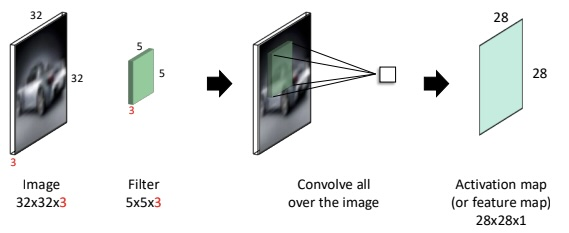
\includegraphics[width=0.8\linewidth]{./img/convolution_filter.jpg}
  \caption{A convolutional filter has the \textbf{same depth} of the input volume, so the output dimension is 1.}
  % \label{fig:forward_mapping}
\end{figure}

We can also train more than one filter, where each filter outputs a feature map.
By stacking activation maps we get a new volume.

Since convolutions shrink the images we can use padding to preserve the edges.
We have always considered a stride of 1 (moving the convolutional filter by one pixel), but we can also use different stride sizes to shrink the image.

\begin{figure}[htbp]
  \centering
  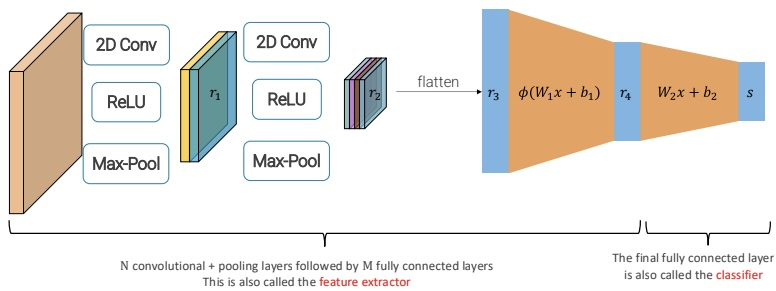
\includegraphics[width=0.8\linewidth]{./img/deep_cnn.jpg}
  \caption{By stacking together convolutional filters, pooling layers and fully connected layers we can design a Deep CNN.}
\end{figure}

\paragraph{Pooling}
A pooling layer is used to reduce the size of the representation in order to speedup computation.
Pooling comes usually after each conv layer or after a block (or set) of conv layers.
It's applied to each activation map independently.

\begin{figure}[htbp]
  \centering
  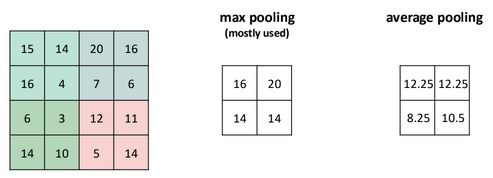
\includegraphics[width=0.6\linewidth]{./img/pooling.jpg}
  \caption{Example: pooling of dimension 2 and stride 2.}
\end{figure}

\paragraph{Receptive fields}
The input pixels affecting a hidden unit are called its receptive field.
We can encode the information in all the pixels to a single point.
We go from spatial to semantic information (we transform spatial information to semantic information).

\paragraph{Convolution parameters and flops}

\begin{figure}[htbp]
  \centering
  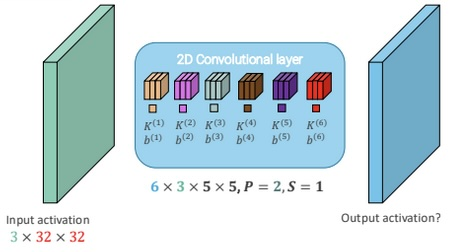
\includegraphics[width=0.6\linewidth]{./img/convolutions_flops.jpg}
%   \caption{}
  \label{fig:convolutions_flops}
\end{figure}

As we can see in \ref{fig:convolutions_flops}, the number of learnable parametes for the convolutional layer is $6 \times (3 \times 5 \times 5 + 1) = 6 \times 76 = 456$ (6 convolutional blocks, 3 channels per convolutional block, $5 \times 5$ convolution, ).
The size of the output is $H_\text{{out}} = W_\text{{out}} = 32 - 5 + 2 * 2 + 1 = 32$.
Hence, there are $6 \times 32 \times 32 = 6144$ values in the output activation ($\approxeq 24$KB).

Each of them is obtained as the dot product between the weights and the input, which requires to perform $n$ multiplications and $n$ summations for inputs of size $n$, i.e. $2n$ flops.

\subsubsection{Batch Normalization (BatchNorm)}
BatchNorm is a technique designed to stabilize and accelerate the training of deep neural networks by addressing internal covariate shift: the change in the distribution of layer activations caused by updates to preceding layers during training.
By normalizing activations at each layer, BatchNorm ensures that gradients are propagated more effectively, enabling coordinated updates across deep networks.

Let $Z^{[l]}$ be a minibatch of activations of the $l$-th layer to be normalized.
To normalize $Z^{[l]}$, we replace it with: $Z^{[l]}_{norm} = \frac{Z^{[l]} - \mu}{\sigma}$, where $\mu$ is a vector containing the mean of each unit and $\sigma$ is a vector containing the standard deviation of each unit.
$\mu$ and $\sigma$ are running averages of the values seen during training.
BatchNorm helps with speeding up the training, and has a slight regularization effect (but we don't use it for this reason).

We use LayerNorm for fully connected layers because it normalizes per sample, making it batch-size independent.
We use InstanceNorm for convolutional layers because it normalizes per sample and per channel.

\subsubsection{Dropout regularization}
Dropout randomly deactivates a fraction of neurons during training, effectively training an ensemble of smaller sub-networks.
For each layer, you set a dropout probability, determining the chance a neuron is ignored in a forward pass.
This helps to prevent overfitting because we don't associate a certain pattern to a certain output of the network.

\begin{figure}[htbp]
  \centering
  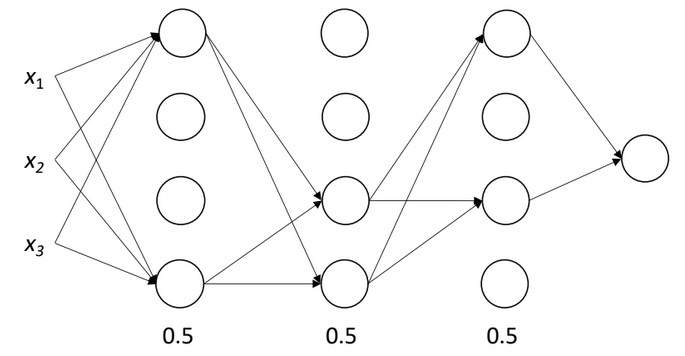
\includegraphics[width=0.6\linewidth]{./img/dropout.jpg}
  \caption{Each layer has a $50 \%$ dropout probability}
  \label{fig:dropout}
\end{figure}

Dropout and normalization are used only at training time.
When we test the network we switch off dropout and regularization.

Another powerful regularization technique is just having more data.

\subsubsection{Data augmentation}
We can create more data by modifying the images we already have.
We must only make transformations which keep the labels valid.
We can, for example, sample random crops/scales of the data or do color augmentation.

Cutout is the process where we remove a random square region of the input image.
This forces the network to use a more diverse set of features, helping generalization.
It's gray because we subtract the mean from this pictures, and so the number in the cutout becomes 0.

\subsection{CNNs}

\subsubsection{AlexNet \& ZFnet}
In 2012 Alex Krizhevsky proposed AlexNet, which had almost a $9\%$ of improvement on SOTA for image classification.

\begin{figure}[htbp]
  \centering
  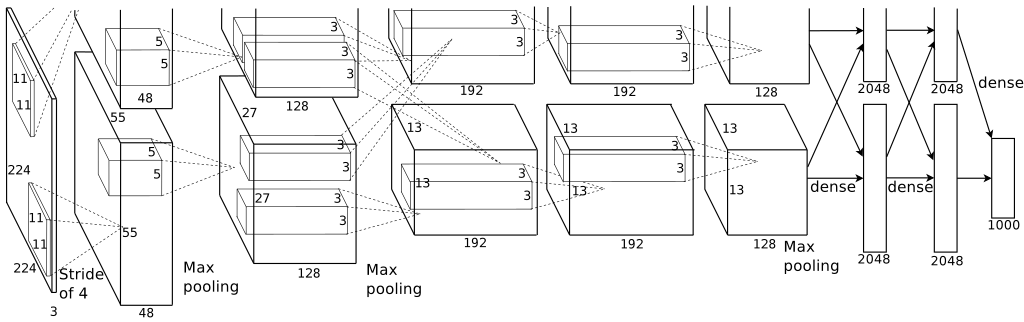
\includegraphics[width=0.8\linewidth]{./img/alexnet.png}
  \caption{AlexNet architecture}
  \label{fig:alexnet}
\end{figure}

In figure \ref{fig:alexnet}, only one half of the network is shown, as the architecture is replicated identically for a 2-GPU setup.

The network begins with a \textbf{stem layer}, which is a convolutional layer that quickly reduces the spatial dimensions of the activations to lower memory and computational requirements.
The first layer uses two $11 \times 11$ kernels to extract features such as corners, edges, and blobs.

However, this design had limitations: the large kernel size ($11 \times 11$) and stride (4) in the first layer caused a significant \textbf{loss of spatial information} early in the network, making it harder to capture fine-grained features.

To address these issues, ZFNet replaced the initial $11 \times 11$ convolutions with $7 \times 7$ convolutions with stride 2 in the first layer, and $5 \times 5$ convolutions with stride 2 in the second layer.

\subsubsection{VGG}
The VGG network architecture is characterized by its simplicity and depth, achieved by exclusively using small $3 \times 3$ convolutional filters and omitting a distinct 'stem' layer. The core structure consists of repeated blocks of convolution and pooling layers, followed by a standard flattening layer and a classification head. Training such deep networks presented challenges, including the vanishing gradient problem. As batch normalization was not yet available during VGG's development, pre-initializing network weights from shallower, pre-trained architectures was a crucial technique for enabling effective training.

\begin{figure}[htbp]
  \centering
  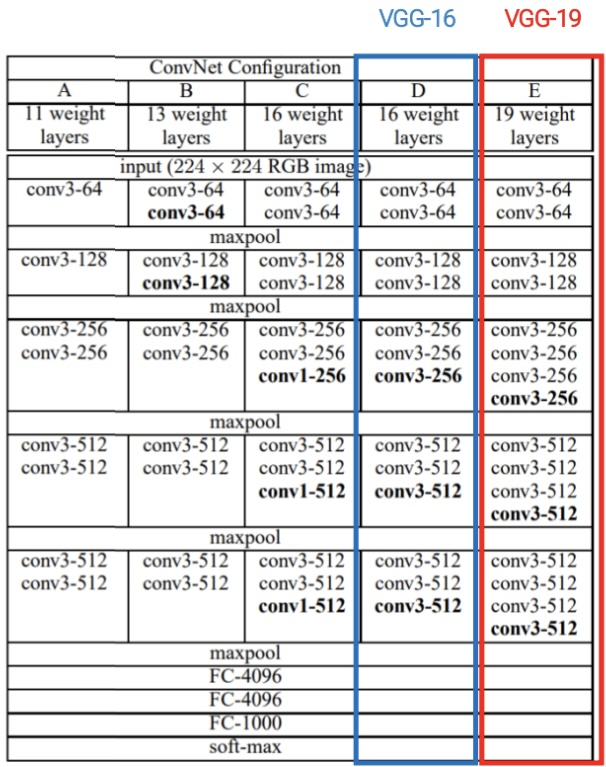
\includegraphics[width=0.45\linewidth]{./img/vgg.jpg}
  \caption{VGG network architecture}
\end{figure}

VGG introduced a modular design principle based on repeating stages. Each stage consists of a fixed sequence of layers that process activations while maintaining the same spatial resolution within that stage. VGG employs three main types of such repeating blocks:
\begin{itemize}
  \item \verb|conv-conv-pool|.
  \item \verb|conv-conv-conv-pool|.
  \item \verb|conv-conv-conv-conv-pool| (we can get a more complex convolution by combining $3\times 3$ convolutions).
\end{itemize}

The use of stacked $3 \times 3$ convolutions within a stage, as detailed in the table below, provides an effective receptive field comparable to that of a single larger convolution (e.g., a $5 \times 5$ filter). However, this approach requires fewer parameters and less computation while also introducing more non-linear activation functions (ReLUs).

A notable trade-off, also highlighted in the table, is the increased memory required for storing activations when using stacked $3 \times 3$ convolutions compared to a single larger filter.

\begin{table}[htbp]
\begin{tabular}{|l|l|l|l|l|}
\hline
convolutional layer                                    & params       & flops                 & ReLUs & number of activations                \\ \hline
$C \times C \times 5 \times 5, \,S=1,\, P=2$           & $25C^2 + C$  & $50C^2 W_{in} H_{in}$ & 1     & $C\times W_{in} \times H_{in}$ \\ \hline
2 stacked $C \times C \times 3 \times 3, \,S=1,\, P=1$ & $18C^2 + 2C$ & $10C^2 W_{in} H_{in}$ & 2     & $2\times C \times W_{in} \times H_{in}$ \\ \hline
\end{tabular}
\end{table}

The VGG-16 model, for instance, comprises 138 million parameters (approximately 2.3 times that of AlexNet), a significant portion of which are in the fully connected layers. It demands considerable computational resources, around 4 TFLOPs, largely due to its convolutional operations, and requires approximately 16.5 GB of memory.

\subsubsection{Inception v1 (GoogLeNet)}
A key feature of this architecture is the efficient use of computational resources within the network. This is achieved through a carefully designed structure that allows for increased depth and width while maintaining a fixed computational budget.

\begin{figure}[htbp]
  \centering
  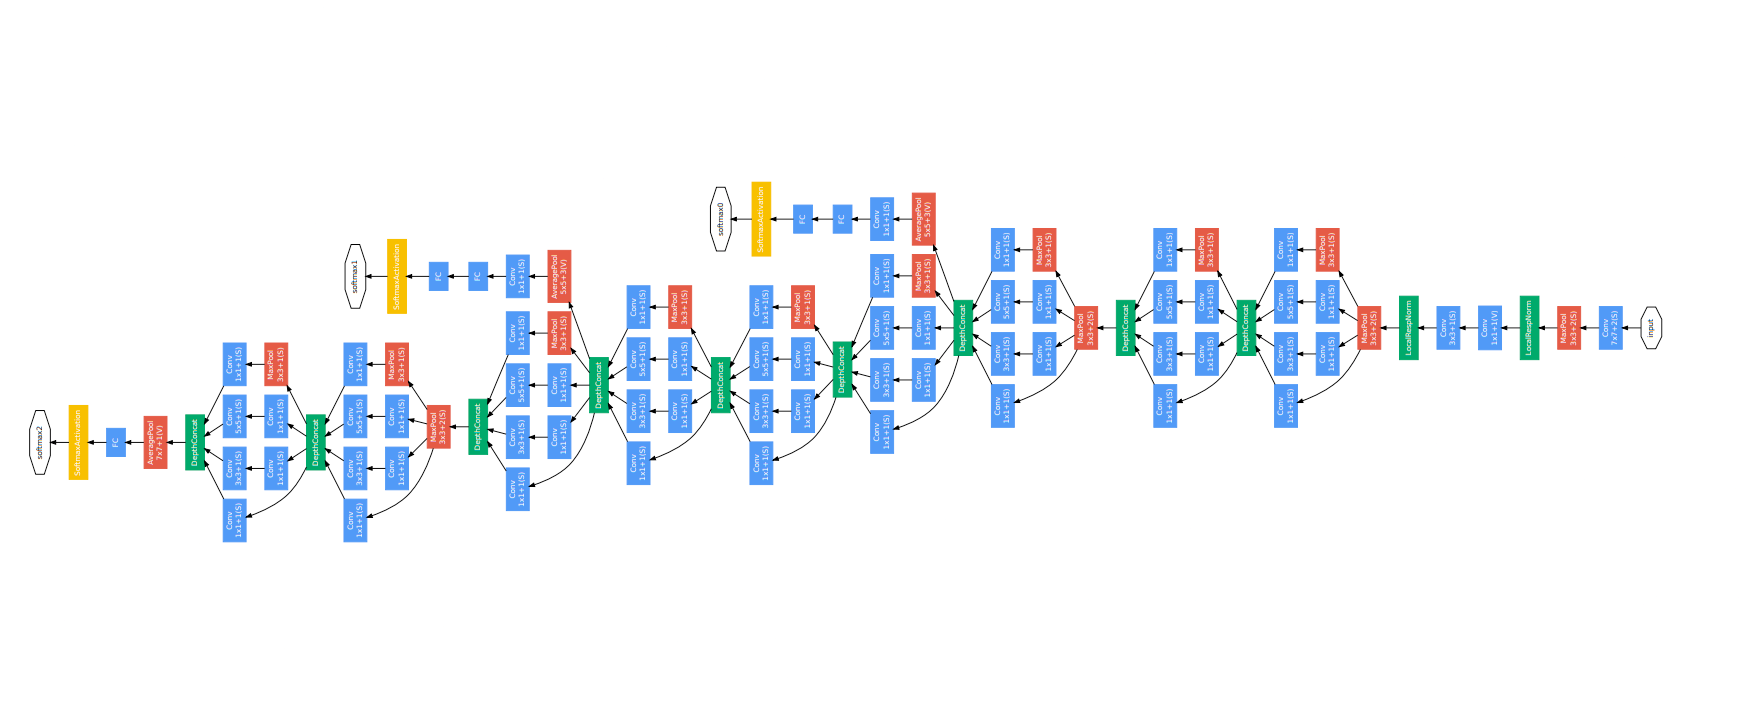
\includegraphics[width=0.99\linewidth]{./img/googlenet.png}
  \caption{GoogLeNet architecture}
\end{figure}

The network consists of stem layers that reduce the input size, a series of inception modules that combine various operations, and a final classifier. It includes 22 trainable layers and roughly 100 modules (represented by the blue and red blocks).

\paragraph{Stem layers}
Stem layers downsample the input aggressively, from 224 to 28 pixels in width/height, within just 5 layers. This approach is slightly more gradual than in AlexNet. For comparison, VGG requires 10 layers to reach a spatial size of $28\times 28$.

\paragraph{Naïve inception module}
The core idea of the inception module is to perform several pooling and convolution operations of different sizes (e.g., $3\times 3$, $5\times 5$) in parallel, rather than using a single type of filter.

\begin{figure}[htbp]
  \centering
  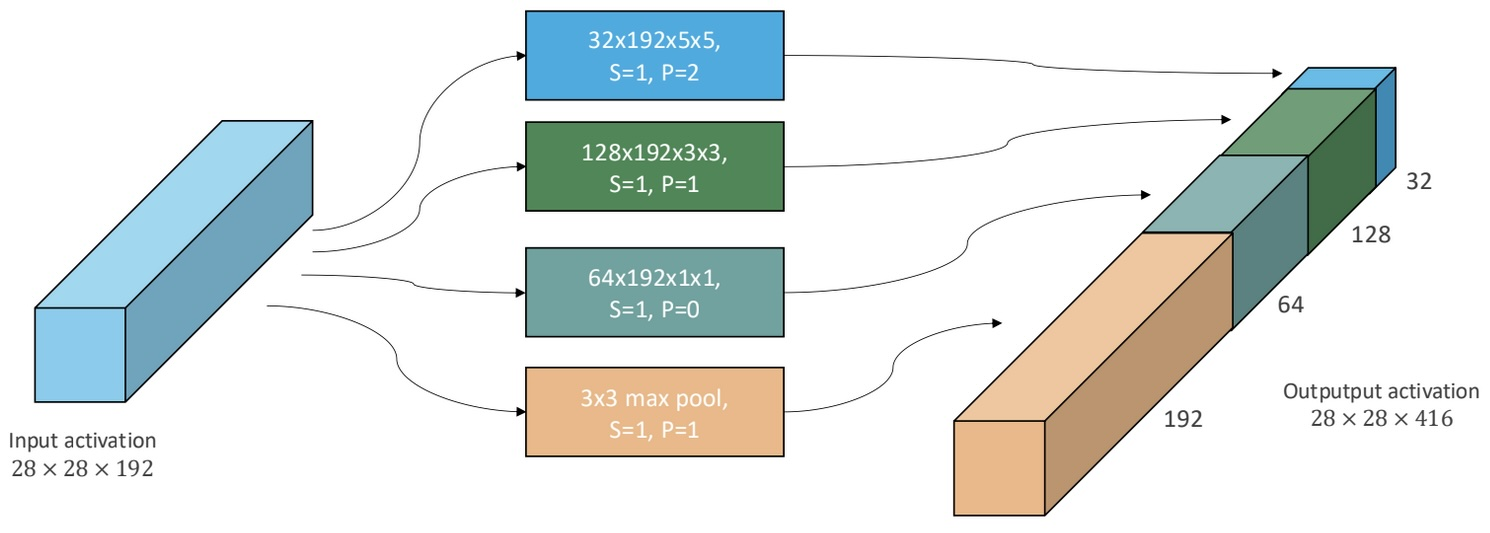
\includegraphics[width=0.7\linewidth]{./img/inception_naive.jpg}
\end{figure}

However, this design introduces two main issues:
\begin{itemize}
  \item The use of max pooling causes the number of channels to grow rapidly when stacking inception modules.
  \item Performing $3 \times 3$ and $5 \times 5$ convolutions on many channels becomes computationally expensive as the network deepens.
\end{itemize}

\paragraph{$1 \times 1$ convolutions and the inception module}
To address these problems, $1 \times 1$ convolutions are applied before the $3\times 3$ and $5\times 5$ convolutions. These $1\times 1$ convolutions do not capture spatial relationships but operate across channels at each spatial location. They enable us to adjust the depth of activations while preserving spatial resolution, effectively serving as a form of dimensionality reduction.

\begin{figure}[htbp]
  \centering
  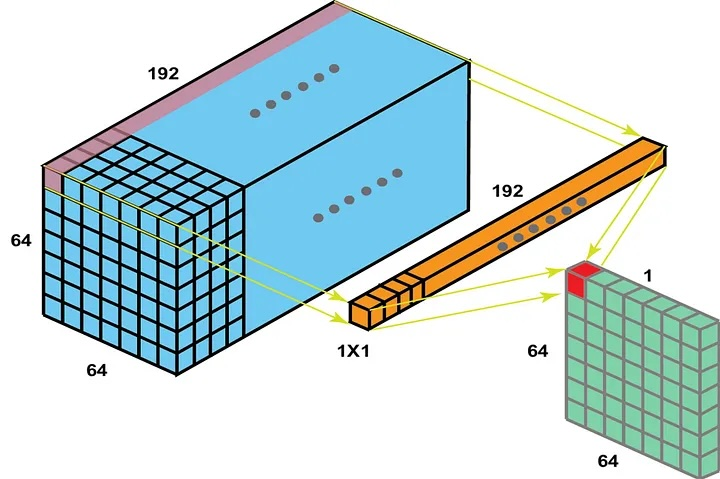
\includegraphics[width=0.6\linewidth]{./img/11conv.jpg}
  \caption{$1 \times 1$ convolution}
\end{figure}

By introducing $1\times 1$ convolutions before the larger convolutions and after pooling, we can:
\begin{itemize}
  \item \textbf{Control time complexity} by reducing the number of channels processed by larger convolutions.
  \item \textbf{Limit the output depth} of the max pooling layers by shrinking the channel dimension.
\end{itemize}

\begin{figure}[htbp]
  \centering
  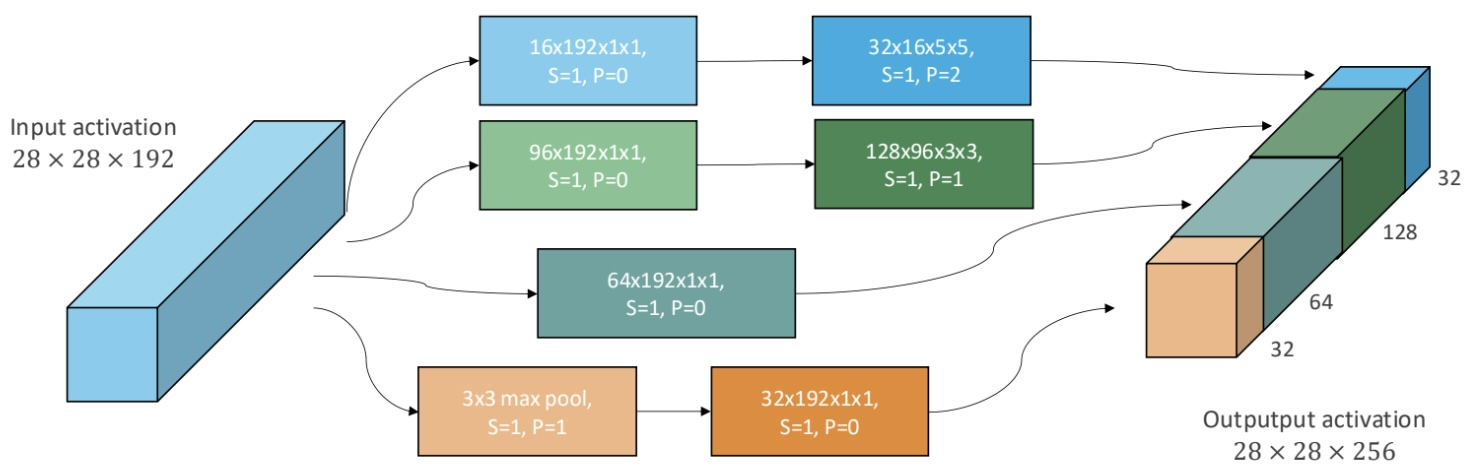
\includegraphics[width=0.8\linewidth]{./img/inception.jpg}
  \caption{Inception module in GoogLeNet}
  \label{fig:inception}
\end{figure}

In Figure~\ref{fig:inception}, we see how Google used $1\times 1$ convolutions to implement an inception module without incurring in excessive computational cost. The approach is to first reduce the number of channels with $1\times 1$ convolutions, then apply the $3 \times 3$ and $5 \times 5$ spatial convolutions. After pooling operations, another $1\times 1$ convolution reduces the output depth. We reduce dimensionality \textbf{after} pooling since compression isn't necessary beforehand.

\paragraph{Fully-connected classifier vs global average pooling}

\begin{figure}[htbp]
  \centering
  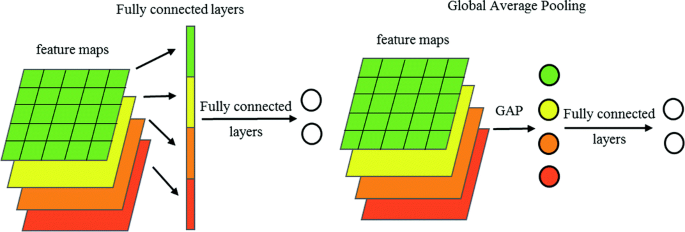
\includegraphics[width=0.6\linewidth]{./img/fc_vs_gap.png}
  \caption{Fully Connected Classifier vs Global Average Pooling}
\end{figure}

The final three fully connected layers typically account for a large portion of the parameters due to high-dimensional spatial inputs. To mitigate this, we eliminate the spatial dimensions by averaging across them. This is justified by the assumption that the final activations represent high-level semantic features.

\subsubsection{Inception v3}
Inception v3 improves computational efficiency and reduces parameter count through convolutional factorization. The two main techniques are:
\begin{itemize}
  \item Replacing a $5 \times 5$ convolution with two sequential $3 \times 3$ convolutions (as in VGG).
  \item Factorizing a $3 \times 3$ convolution into a $3\times 1$ followed by a $1 \times 3$ convolution.
\end{itemize}

\begin{figure}[htbp]
  \centering
  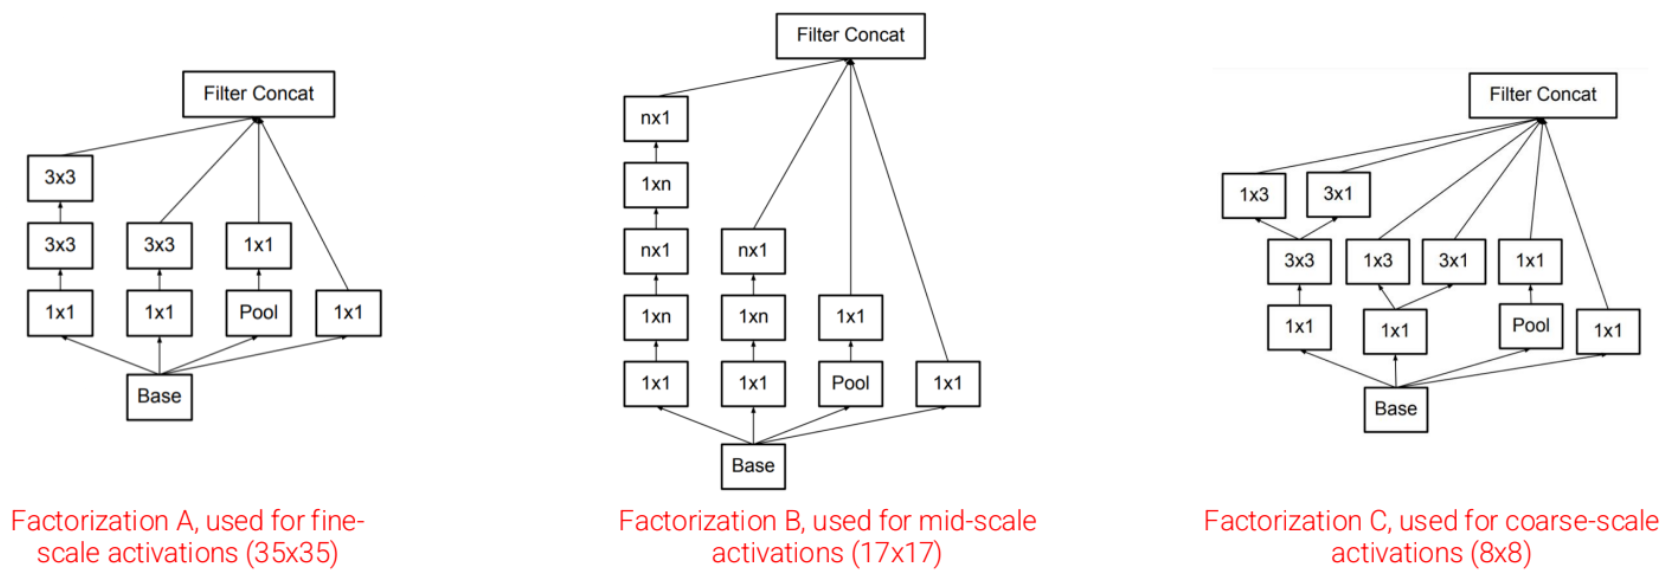
\includegraphics[width=0.8\linewidth]{./img/inception3.png}
  \caption{Inception v3 uses three different types of inception layers instead of a single repeated one}
\end{figure}

\subsubsection{Residual Networks (ResNet)}
ResNet was designed to solve two major problems in deep neural networks: the vanishing gradient problem and degradation (when adding more layers actually makes performance worse). 

The key idea behind ResNet is the \textbf{residual block}, which includes a \textbf{skip connection}. In standard networks, each layer passes its output directly to the next layer. In ResNet, the input to a layer is also added to its output:
\[
H(x) = F(x) + x
\]
This means the network learns the residual function $F(x) = H(x) - x$, which is easier to optimize.

\begin{figure}[htbp]
  \centering
  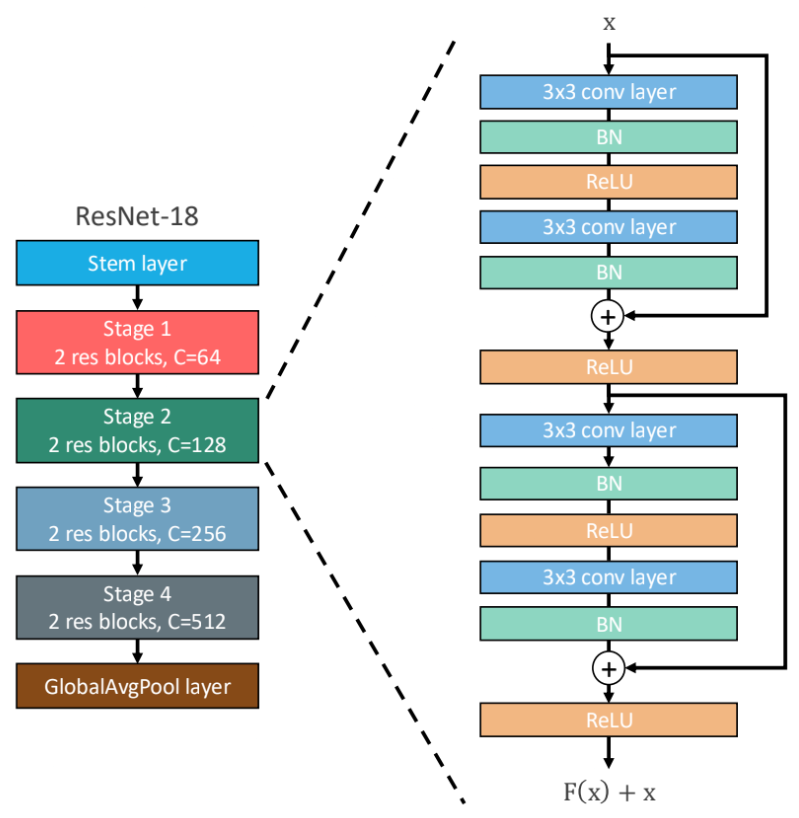
\includegraphics[width=0.4\linewidth]{./img/resnet.png}
  \caption{The ResNet architecture}
\end{figure}

ResNet architecture follows a structured pattern, inspired by VGG:
\begin{itemize}
  \item Each \textbf{stage} is made up of multiple residual blocks.
  \item Each residual block contains two $3 \times 3$ convolutional layers, each followed by batch normalization.
  \item The first block of each stage reduces the spatial resolution (via stride 2) and doubles the number of channels.
  \item The network starts with a stem layer and ends with global average pooling, like GoogLeNet.
\end{itemize}

\begin{figure}[htbp]
  \centering
  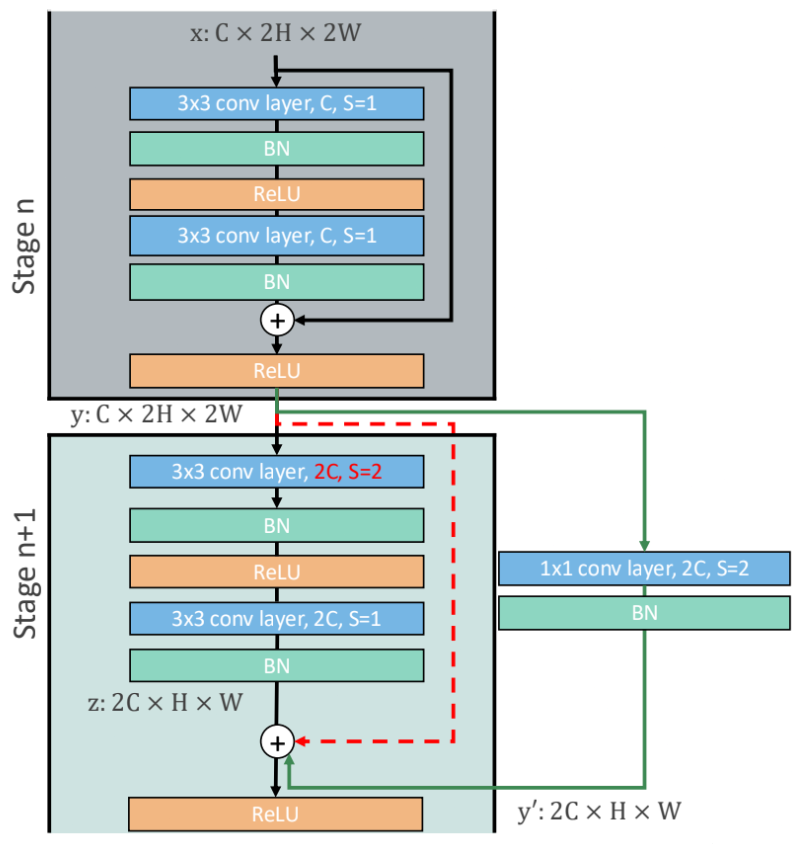
\includegraphics[width=0.4\linewidth]{./img/resnet_skip.png}
\end{figure}

ResNet remains a standard baseline in many computer vision tasks.

\paragraph{Handling dimension mismatch}
Residual blocks cannot be directly used at the start of a new stage, since the number of channels and spatial resolution change. To handle this, ResNet uses a $1 \times 1$ convolution with stride 2 to match dimensions across the skip connection.

\paragraph{Bottleneck Residual Block}
For deeper networks like ResNet-50/101/152, a \textbf{bottleneck block} is used to reduce computational cost. Instead of stacking two $3 \times 3$ convolutions, the bottleneck design compresses and then expands channels:
\begin{itemize}
  \item $1 \times 1$ conv to reduce dimensions from $4C$ to $C$
  \item $3 \times 3$ conv processes $C$ channels
  \item $1 \times 1$ conv expands back to $4C$
\end{itemize}

\begin{figure}[htbp]
  \centering
  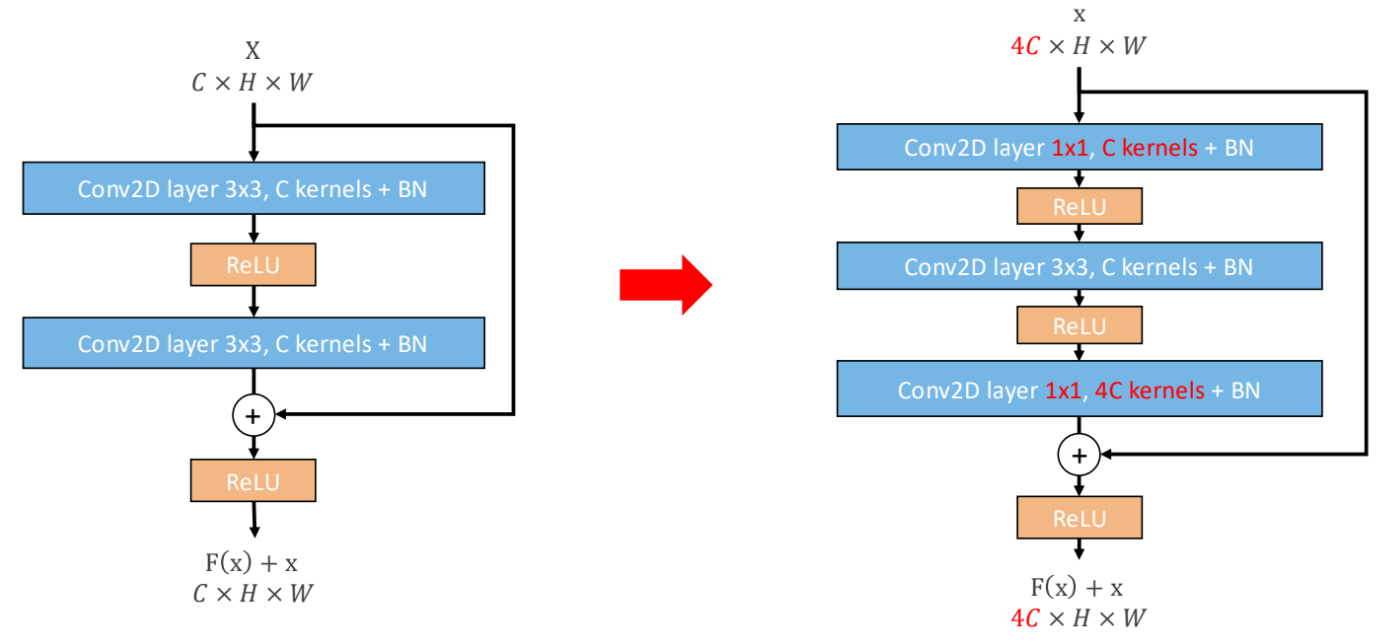
\includegraphics[width=0.8\linewidth]{./img/resnet_bottleneck.png}
  \caption{Bottleneck residual block}
\end{figure}

\subsubsection{ResNeXt}
ResNeXt builds on ResNet but introduces a new dimension: \textbf{cardinality}, which is the number of parallel paths or groups.

\begin{figure}[htbp]
  \centering
  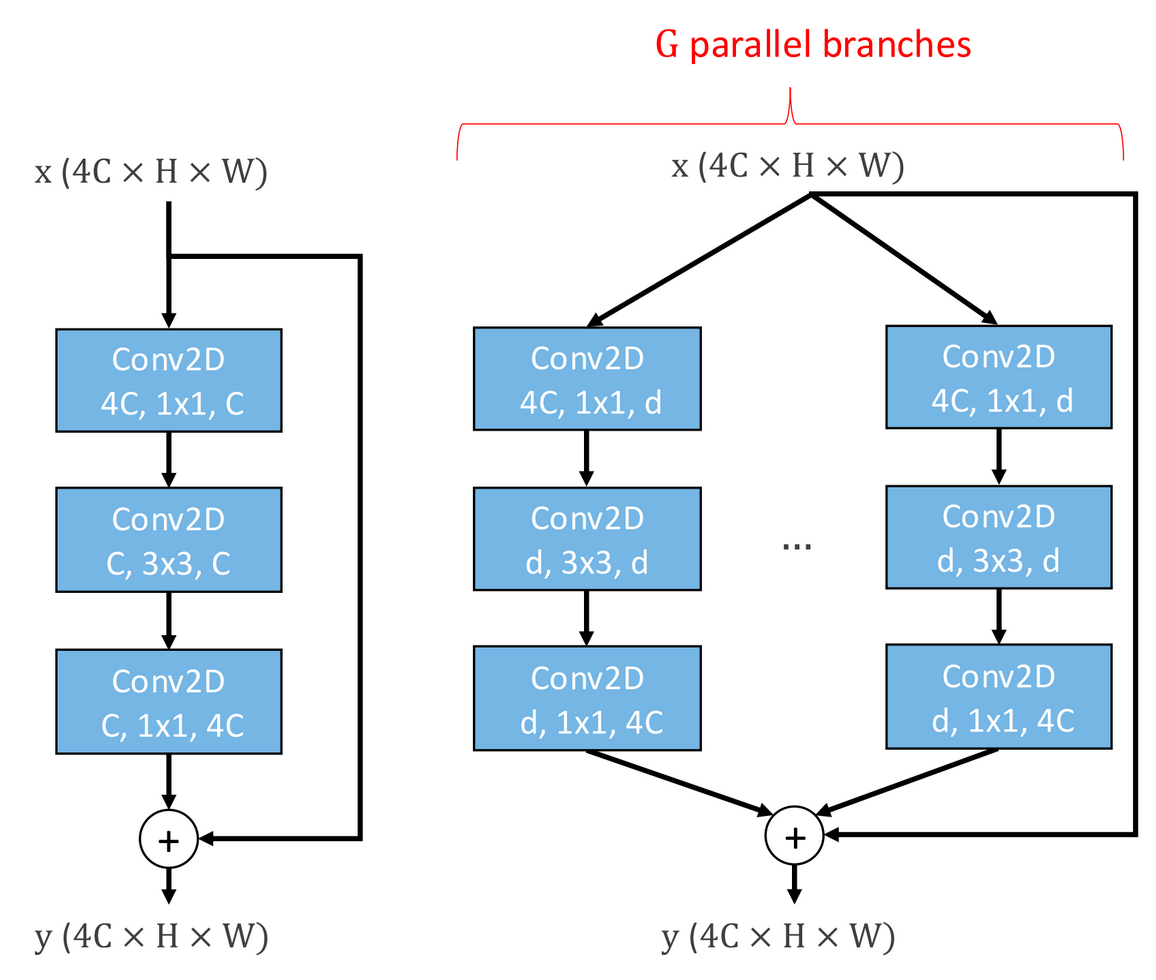
\includegraphics[width=0.5\linewidth]{./img/resnext.png}
  \caption{ResNeXt network architecture}
\end{figure}

Inspired by Inception modules (which split-transform-merge), ResNeXt uses multiple paths inside each residual block. Each block is split into $G$ branches (cardinality), and each branch learns part of the features.

The ResNeXt block is a simplified and efficient version of multi-branch architecture.

\paragraph{Grouped Convolutions}
Each branch is implemented using \textbf{grouped convolutions}:
\begin{itemize}
  \item The input with $C$ channels is split into $G$ groups, each with $\frac{C}{G}$ channels.
  \item Each group has separate filters, and processes data independently.
  \item The outputs of all groups are concatenated, giving $K$ total channels (for $K$ filters).
\end{itemize}

\begin{figure}[htbp]
  \centering
  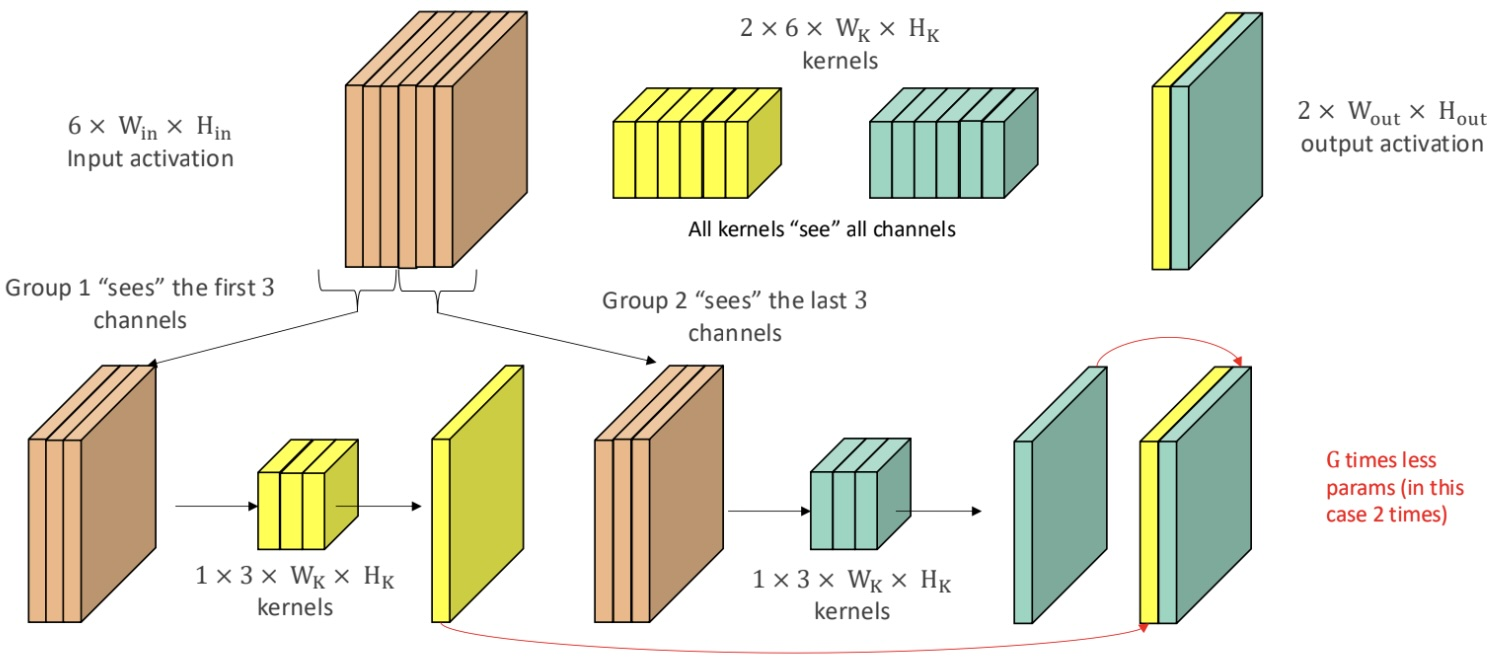
\includegraphics[width=0.6\linewidth]{./img/grouped_convolutions.jpg}
  \caption{Grouped convolution in ResNeXt with $G=2$}
\end{figure}

\paragraph{Structure of a ResNeXt Block}
\begin{itemize}
  \item $1 \times 1$ convolution to reduce input channels.
  \item $3 \times 3$ grouped convolution processes features in $G$ groups.
  \item $1 \times 1$ convolution expands channels back.
  \item Skip connection adds the original input.
\end{itemize}

\begin{figure}[htbp]
  \centering
  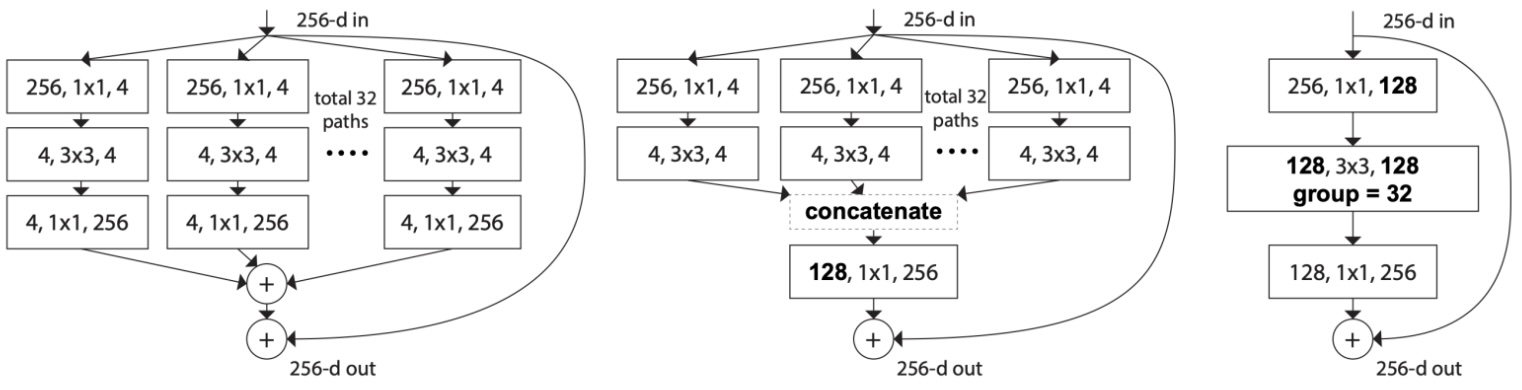
\includegraphics[width=0.85\linewidth]{./img/resnext_grouped.jpg}
  \caption{ResNeXt block with grouped convolutions: split, transform, merge.}
\end{figure}

\textbf{Why ResNeXt?}  
It improves performance with fewer parameters and less computation than simply increasing network depth or width. Increasing cardinality $G$ enhances feature learning efficiency without a significant cost in resources.

\subsubsection{Squeeze-and-Excitation Networks (SENet)}
It's the last paper which won CVPR.
It proposed the squeeze-and-excitation module to capture global context and to use it to reweight channels in each block.
Given the output $U$ of a block with shape $C \times H \times W$ we do:
\begin{itemize}
  \item Global average pooling to squeeze.
  \item General bottleneck formed by two fully connected layers with reduction ratio 16.
\end{itemize}

\begin{figure}[htbp]
  \centering
  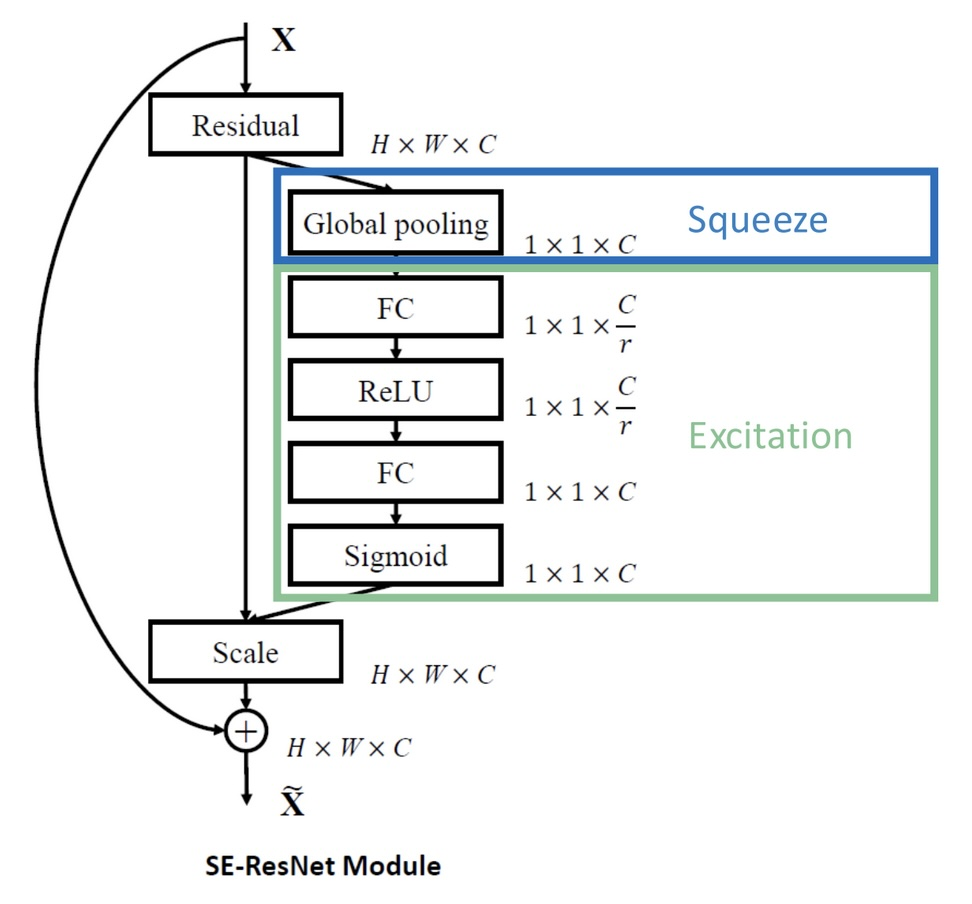
\includegraphics[width=0.5\linewidth]{./img/senet.jpg}
  \caption{SENet network block diagram}
\end{figure}

\subsubsection{Depthwise Separable convolutions}
F. Chollet one year after the SENet paper proposed the Depthwise Separable convolutions.
The standard convolutions filter features based on the convolutional kernels and combine features in order to produce new representations.
This is very expensive.
Depthwise separable convolutions separates filtering and combination, and this aggressively limits the computational cost.

\begin{figure}[htbp]
  \centering
  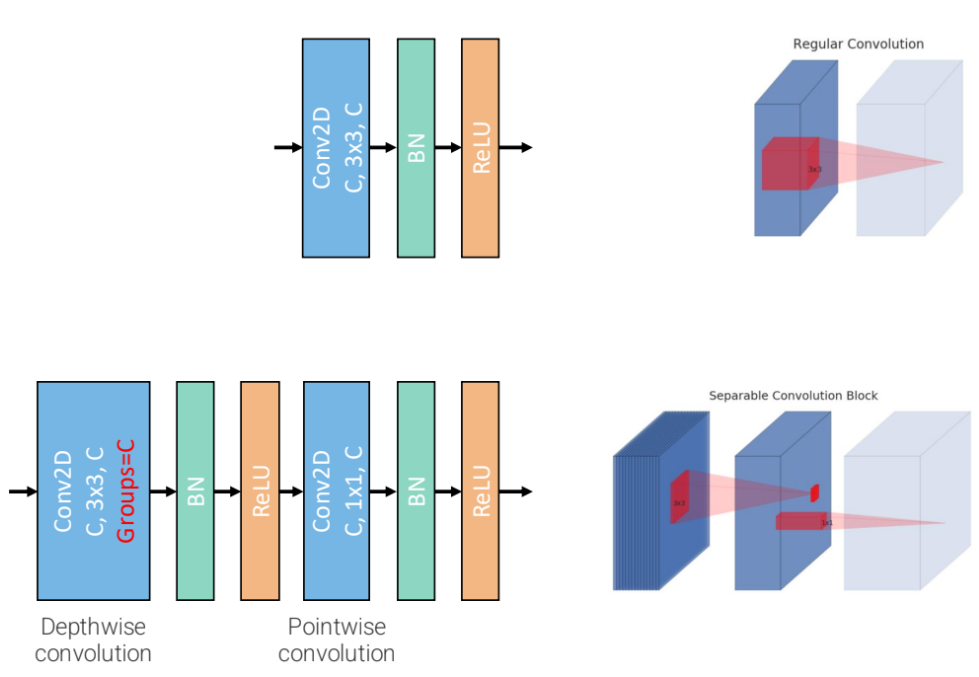
\includegraphics[width=0.5\linewidth]{./img/separable_convolution.png}
  \caption{Depthwise Separable convolutions}
\end{figure}

\subsubsection{Inverted residual blocks}
MobileNet-v2 introduced the bottleneck residual block to scale up the model depth by increasing the number of layers per block while keeping the computation and number of parameters roughly constant.
To this end, it uses a pair of $1\times 1$ convolutions, where the first compresses the number of channels, while the second one expands them.
Hence, the $3\times 3$ convoltuion operates in the compressed domain.

\begin{figure}[htbp]
  \centering
  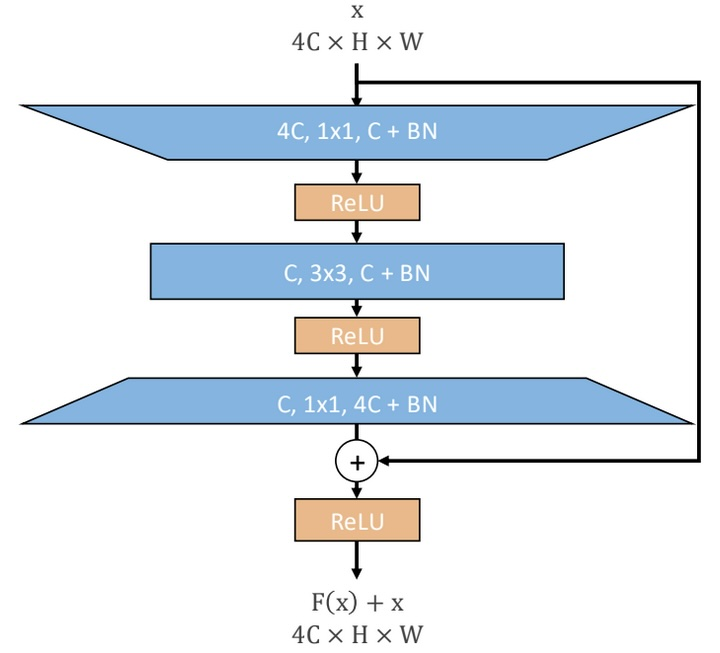
\includegraphics[width=0.4\linewidth]{./img/bottleneck_residual.jpg}
  \caption{Bottleneck residual block}
\end{figure}

As we know, compression usually results in information loss, so in MobileNet-v2 inverted residual blocks were proposed.
In this blocks, the first $1\times 1$ convolution expands the channels, while the second compresses them back, according to an expansion ratio $t$.
To limit the increase in computation, the inner $3\times 3$ convolution is realized as a depthwise convolution (single filter per input channel instead of applying the filters across all the input channels).

\begin{figure}[htbp]
  \centering
  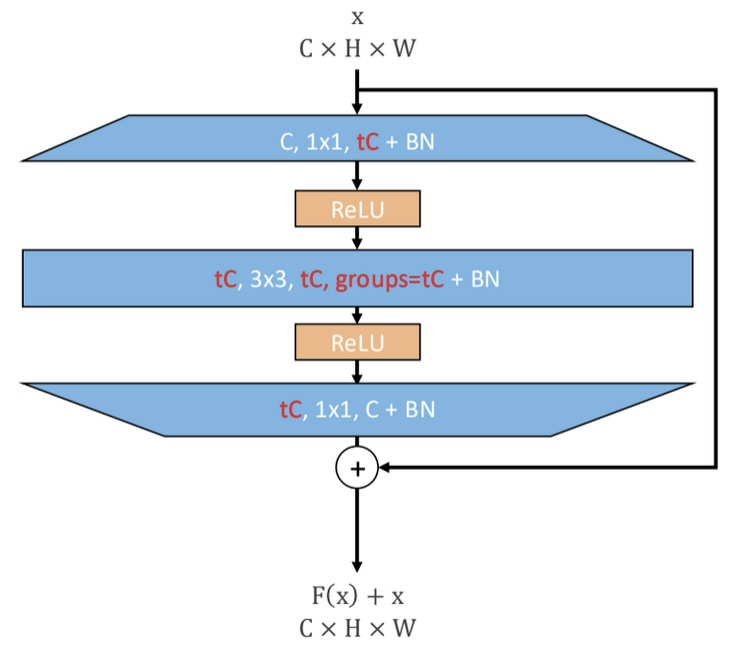
\includegraphics[width=0.4\linewidth]{./img/inverted_residual.jpg}
  \caption{Inverted residual block}
\end{figure}

\subsubsection{MobileNet-v2}
MobileNet-v2 is a stack of inverted residual blocks with ReLUs in between.
The number of channels grows slowly compared to previous architectures, as we can see in the purple rectangle in figure \ref{fig:mobilenet}

\begin{figure}[htbp]
  \centering
  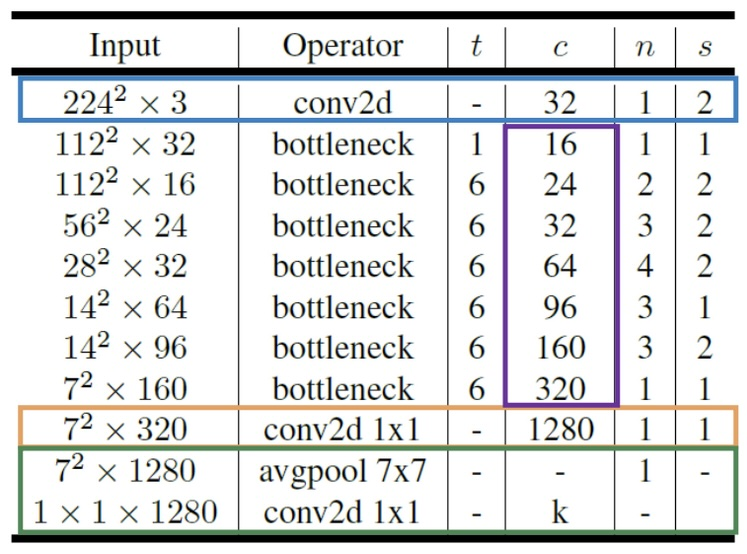
\includegraphics[width=0.5\linewidth]{./img/mobilenet.jpg}
  \caption{Mobilenet network architecture}
  \label{fig:mobilenet}
\end{figure}

Whenever spatial dimensions or number of channels do not match between input and output, there are no residual connections.

\subsubsection{EfficientNet}
EfficientNet proposes designing the network based on available computational resources.  
There are three main dimensions for scaling a neural network: width, depth, and input resolution.

\begin{figure}[htbp]
  \centering
  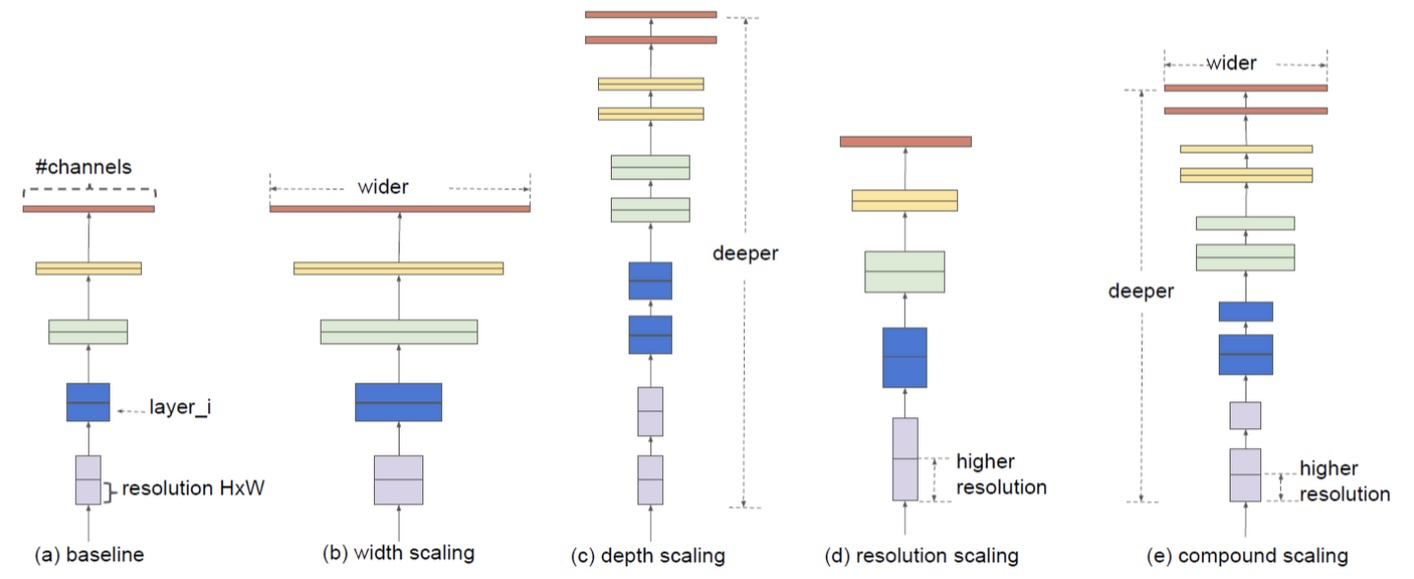
\includegraphics[width=0.9\linewidth]{./img/efficientnet.jpg}
  \caption{Different types of neural network scaling.}
\end{figure}

Larger networks with greater width, depth, or resolution tend to achieve higher accuracy. However, the accuracy gains quickly saturate after around $80\%$, highlighting a limitation of scaling along a single dimension.  
\textbf{The scaling dimensions are not independent.} Intuitively, when increasing image resolution, we should also increase network depth so that larger receptive fields can capture relevant features spanning more pixels.  
Similarly, increasing width becomes important at higher resolutions to capture fine-grained patterns present in the additional pixel information.

EfficientNet addresses this by using a compound coefficient $\phi$ to scale all three dimensions in a balanced and principled way.

\subsection{RNNs \& Transformers}

In RNNs, which were used to avoid the problem of fixed size input, the gradient computation involves performing a forward propagation pass moving from left to right through the unrolled graph of the network, followed by a backward propagation pass moving right to left through the graph.
The basic problem is that by propagating the gradient over many stages it tends to vanish or explode, so learning long-term dependencies can take a lot of time.

\paragraph{Encoder-Decoder architecture}
In this type of architecture the encoder processes the input sequence.
It emits the context $C$, usually as a function of its final hidden state.
The decoder is conditioned on that fixed-length vector to generate the output sequence.
If the context $C$ is a vector, then the encoder RNN is simply a sequence-to-vector RNN, and the decoder is a vector-to-sequence RNN.
The \textbf{bottleneck problem} arises because the context $C$ outputted by the encoder RNN has a dimension that is too small to properly summarize a long sequence.

\paragraph{Attention}
Existing models for neural machine translation encode a source sentence into a fixed-length vector from which a decoder generates a translation.
Attention provides a solution to the bottleneck problem. 
We provide to the decoder the learned token start, then we do the dot product between the start token and the hidden states.
All the other hidden states give us a probability for each token.

\begin{figure}[htbp]
  \centering
  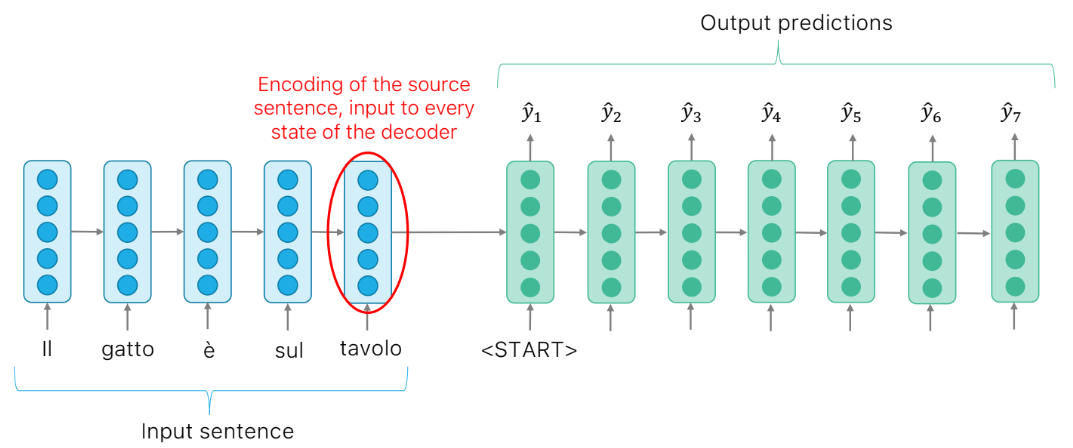
\includegraphics[width=0.7\linewidth]{./img/rnn_classic.png}
  \caption{In the classic RNN, the last hidden state is used for all the translation.}
\end{figure}

\begin{figure}[htbp]
  \centering
  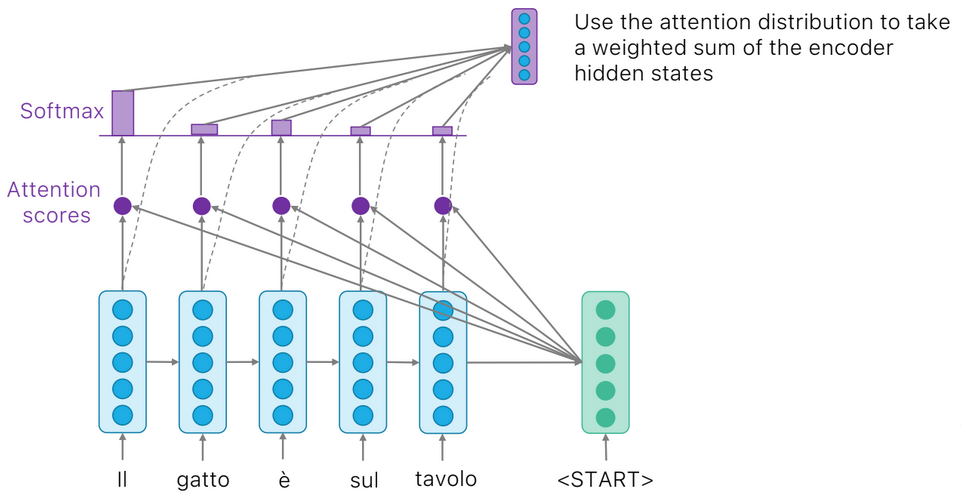
\includegraphics[width=0.7\linewidth]{./img/attention.png}
  \caption{In the attention mechanism, at each step, the current hidden state is compared with all the previous hidden states by computing an attention score.}
\end{figure}

\subsubsection{Transformer architecture}
The inherently sequential nature of RNN precludes parallelization within training examples, which becomes critical with longer sequence lengths.
The \textbf{transformer} is the first model relying entirely on self-attention (and cross-attention) to compute representations of its input and output without using RNNs or convolutions.
It's still an encoder-decoder architecture, where the encoder maps an input sequence of symbol representations $(x_1, ..., x_n)$ to a sequence of continuous representations $z=(z_1, ..., z_n)$.
Given $z$, the decoder generates an output sequence $(y_1, ..., y_m)$ of symbols one element at a time.
At each step the model is \textbf{auto-regressive}, consuming the previously generated symbols as additional input when generating the next.

\begin{figure}[htbp]
  \centering
  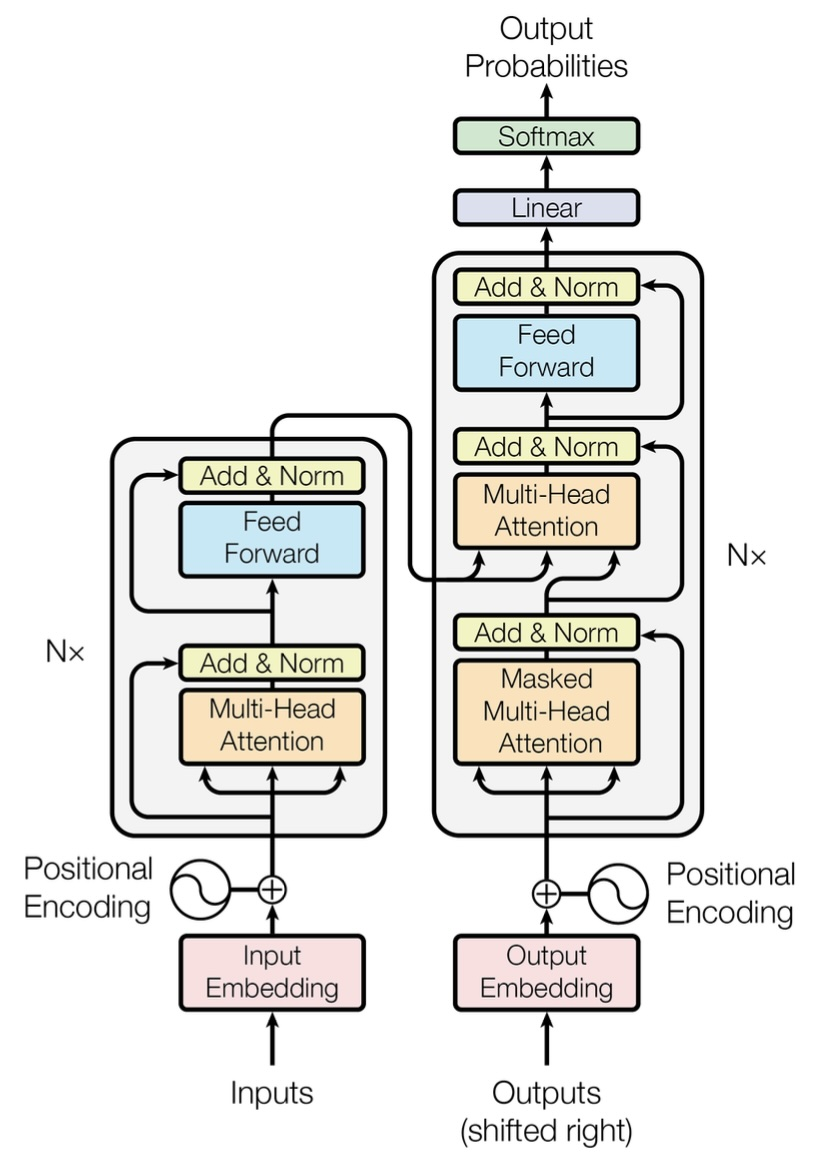
\includegraphics[width=0.6\linewidth]{./img/transformer.jpg}
  \caption{The transformer architecture from the paper "Attention is all you need".}
\end{figure}

\paragraph{Transformer encoder}
In the encoder we turn each input word into a vector by using an embedding layer.
Each word is embedded into a vector of size $d_{\text{model}}$.
If the encoders are stacked, the embedding only happens in the bottom-most encoder.
Since we process the words in parallel we lose positional information, so by using positional encoding we keep this information.
The positional encoding has the same dimension $d_{\text{model}}$ as the embeddings, so that the two can be summed.
There are learned and fixed positional encodings; the authors used sine and cosine functions of different frequencies.

Each layer has two sub-layers:
\begin{itemize}
  \item A multi-head self attention mechanism.
  \item A fully connected feed-forward network. The exact same feedforward network is independently applied to each position (shared parameters).
\end{itemize}

There is also a residual connection around each of the two sub-layers, followed by layer normalization.
To facilitate these residual connections, all sub-layers in the model, as well as the embedding layers, produce outputs of dimension $d_{\text{model}}$.

\paragraph{Transfromer decoder}
The decoder is also composed of a stack of $N$ identical layers.
In addition of the two sub-layers of the encoder, the decoder has a third sub-layer, which performs multi-head attention over the output of the encoder stack (cross-attention).
As in the encoder there are residual connections and layer normalization.

The self-attention sub-layer in the decoder stack is modified so as to \textbf{prevent positions from attending to subsequent positions}.
This masking, combined with the fact that the output embeddings are offset by one position, ensures that the predictions for position $i$ can depend only on the known outputs at positions less than $i$.

\paragraph{Self-Attention}
The first setp in calculating self-attention is to create three vectors from each of the embedded words:
\begin{itemize}
  \item a Query vector.
  \item a Key vector.
  \item a Value vector.
\end{itemize}

These vectors are created by multiplying the embeddings by three matrices learned during the training process.
Their dimensionality is $d_k = \frac{d_{\text{model}}}{h}$, while the embedding and encoder input/output vectors have dimensionality of $d_{\text{model}}$.

The matrices are used to compute the self-attention score.
$$\text{Attention}(Q,K,V)=\text{softmax}(\frac{QK^T}{\sqrt{d_k}})V$$

As we can see there is a little normalization done with $\sqrt{d_k}$, to try to avoid having the results of the softmax squeezed too much into a single value (one hot).
The scores of the self-attention determine how much focus to place on other parts of the input sentence as we encode a word at a certain position.

\paragraph{MultiHead Attention}
The purpose of multi-head attention is to linearly project the queries, keys and values $h$ times with different, learned linear projections.
On each of these projected versions of queries, keys, and values we perform the attention function in parallel.
The outputs of different heads are then concatenated and once again projected.
Multi-head attention allows the model to jointly attend to information from different representation subspaces at different positions.

% \paragraph{Multi Head Self-Attention computation}

\paragraph{Cross-Attention}
in the cross attention layers, the queries come from the previous decoder layer (masked self-attention), and the keys and values come from the output of the encoder.
This allows every position in the decoder to attend over all positions in the input sequence.
It's a very powerful mechanism used in modern generative models to introduce variable lengths conditions.


\subsubsection{Vision Transformer (ViT)}
We split an image into patches and provide the sequence of linear embeddings of these patches as an input to a Transformer.
The image patches are treated the same way as tokens in an NLP application.

As an alternative to raw image patches, the input sequence can be formed from feature maps of a CNN.
In this hybrid model, the patch embedding projection is applied to patches extracted from a CNN feature map.

To handle $2D$ images, we reshape the image $x \in \mathbb{R}^{H\times W \times C}$ into a sequence of flattened $2D$ patches $x_p \in \mathbb{R}^{N \times (P^2 \cdot C)}$.
\begin{itemize}
  \item $(H, W)$ is the resolution of the original image.
  \item $C$ is the number of channels.
  \item $(P, P)$ is the resolution of each image patch.
  \item $N = \frac{HW}{P^2}$ is the resulting number of patches, which also serves as the effective input sequence length for the transformer.
\end{itemize}

The transformer uses constant latent vector size $d_{\text{model}}$ through all of its layers, so we flatten the patches and map to $d_{\text{model}}$ dimensions with a trainable linear projection.
We also prepend a learnable embedding to the sequence of embedded patches, whose state at the output of the transfromer encoder serves as the image representation.
The classification head is implemented by a MLP with one hidden layer.
To retain positional information the ViT uses learnable 1D position embeddings.

\begin{figure}[htbp]
  \centering
  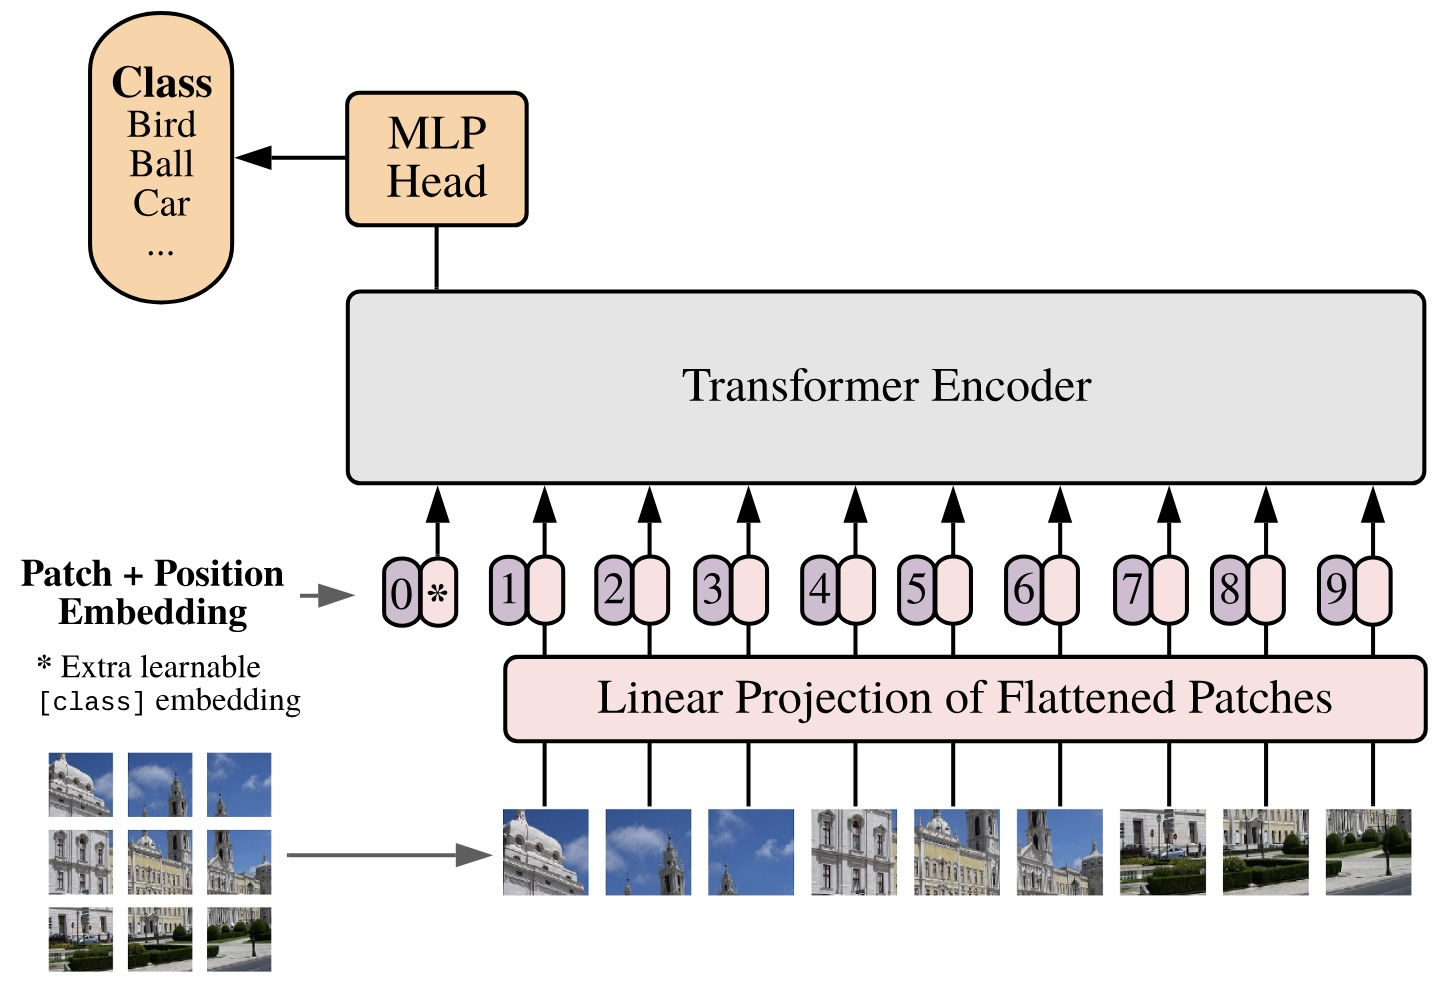
\includegraphics[width=0.6\linewidth]{./img/vision_transformer.jpg}
  \caption{Vision transformer model overview. We split an image into fixed-size patches, linearly embed each of them, add position embeddings, and feed the resulting sequence of vectors to a standard Transformer encoder. In order to perform classification, we use the standard approach of adding an extra learnable “classification token” to the sequence.}
\end{figure}

At the start, the ViT worked very bad.
This is because transformers lack some of the inductive biases inherent to CNNs, such as translation equivariance and locality, and therefore do not generalize well when trained on insufficient amounts of data.
The convolution in combination with max pooling/striding makes CNNs approximately invariant to translation.
When a module is translation invariant, it means that if we apply translation transformation on the input image the output of the module won't change.
To solve the inductive bias they gave the network so much data that the classes appear anywhere.

\subsection{Object Detection}
Previously, we have done object detection with SIFT, but we were just able to say if the object was in the image, not where it was.
Now we want to do detection by putting a bounding box around the object.
We do this by returning a set of quadruples: $[x, y, h, w, o]_{i=0}^{K}$, where we have the box position, width, height, and class of the output.

The main challenges are the different lengths of the outputs (since we can detect from 0 to $K$ images), the fact that the outputs have both categorical and spatial information, and the fact that the images are usually processed at higher resolution than neural networks for image classification.

\subsubsection{Viola-Jones Object Detector}
It's a general purpose object detection framework, but it has been mainly applied to faces.
We will now see the three main innovations of the algorithm: the AdaBoost algorithm, cascade, and the use of integral images.

\paragraph{AdaBoost algorithm}
A Weak Learner (WL) is a simple classifier whose error is slightly better than random guessing.
Boosting is a way to train and build an ensemble of $M$ weak classifiers to obtain a Strong Learner SL.
After training a weak learner, the examples are re-weighted in order to emphasize those which were incorrectly classified by the previous weak classifier.

The \textbf{AdaBoost} algorithm steps are:
\begin{enumerate}
  \item Given $N$ training samples $(x^{(i)}, y^{(i)})$, assign equal weight to each training example $w^{(i)}=\frac{1}{N}$.
  \item Iterate for $j = 1, ..., M$ weak learners:
  \begin{enumerate}
    \item Fit the best classifier $WL_j$ to the training data by using the current weights.
    \item Compute the weighted error rate $\epsilon_j = \sum_{i:\, x^{(i)} \text{ is missclassified}} w^{(i)}$.
    \item Compute $\beta_j = \frac{1 - \epsilon_j}{\epsilon_j}$.
    \item Updates weights $w^{(i)} = w^{(i)}\beta_j$ for wrongly classified examples.
    \item Re-normalize $w^{(i)}$ to sum to 1.
  \end{enumerate}
  \item The Strong Learner is given by a weighted majority vote $SL(x) = \sum_{j} \ln \beta_j WL_j(x) > 0$, con $\ln \beta_j = \alpha_j$.
\end{enumerate}

The idea is that missclassified examples gain weight, forcing subsequent learners to focus on harder cases.

\paragraph{Haar-like features}
Weak classifiers used to detect faces are simple rectangular filters, composed of 2 to 4 rectangles applied at a fixed position within a $24 \times 24$ patch.
Even with this simple definition there are over $160$ k possible filters in a $24 \times 24$ patch.
AdaBoost is used to select a small subset of the most effective filters.

\paragraph{Dataset}
The dataset consisted of 4916 hand labeled faces, scaled and aligned to a base resolution of $24 \times 24$ pixels.
The non-face windows were collected by selecting random sub-windows from a set of 9500 images which did not contain faces.

\begin{figure}[htbp]
  \centering
  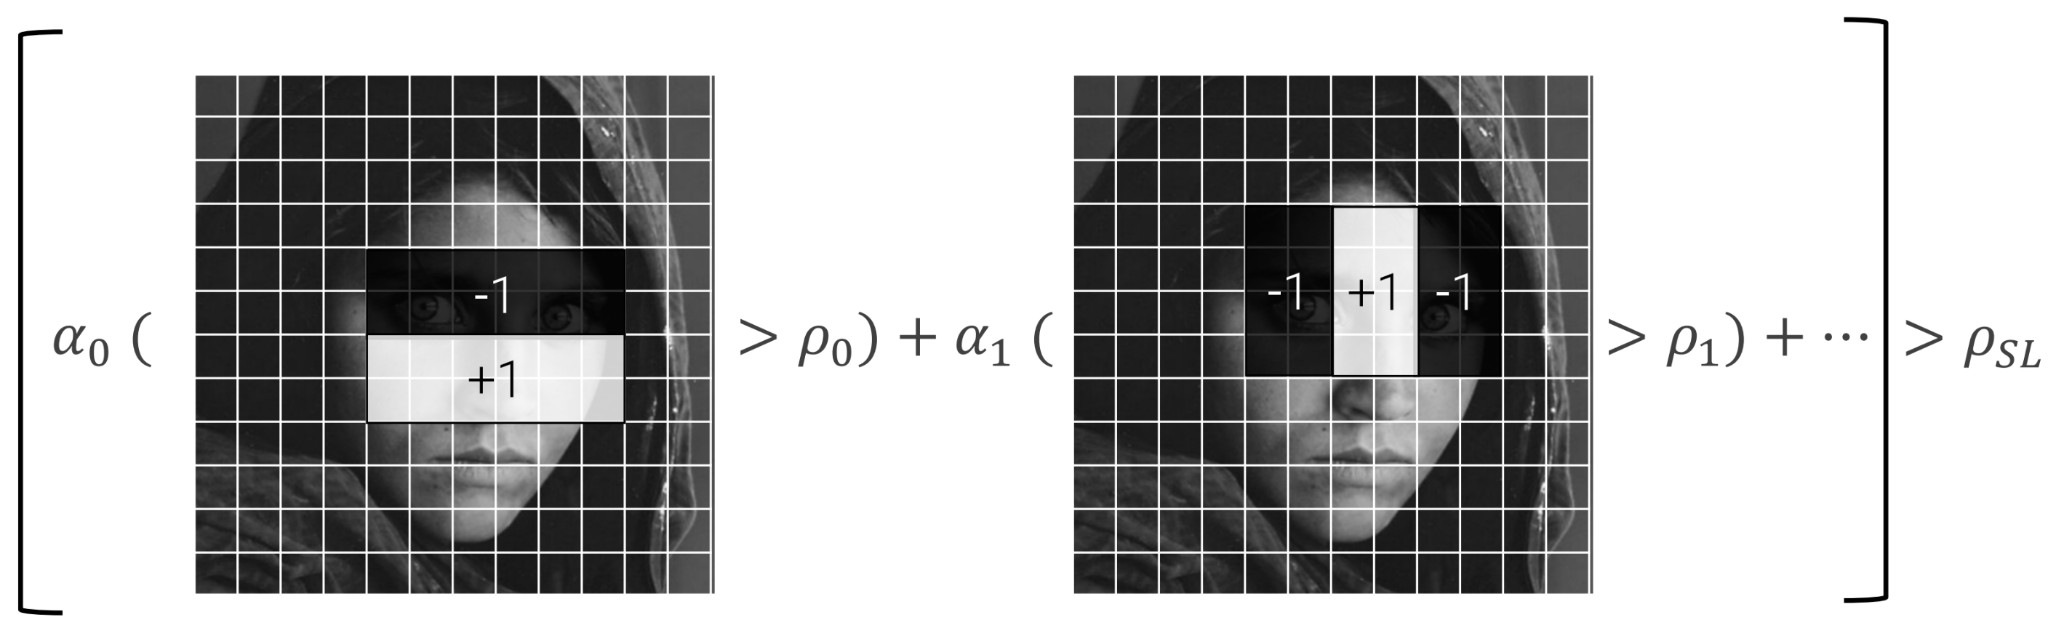
\includegraphics[width=0.6\linewidth]{./img/adaboost.png}
  \caption{The 2 most effective features selected by AdaBoost on the training set.}
\end{figure}

\paragraph{Integral images and fast feature computation}
To speed up the computation of rectangular features, the authors proposed the use of so-called integral images $II$, where $II(i,j) = \sum_{i' \leq i, j' \leq j} I(i', j')$.

We can compute the value of $II(i,j)$ just by looking at the 3 neighbors: $II(i,j) = II(i, j-1) + II(i-1, j) - II(i-1, j-1) + I(i,j)$, where $II$ are the values in the integral image, and $I$ is the value in the original image.

\begin{figure}[htbp]
  \centering
  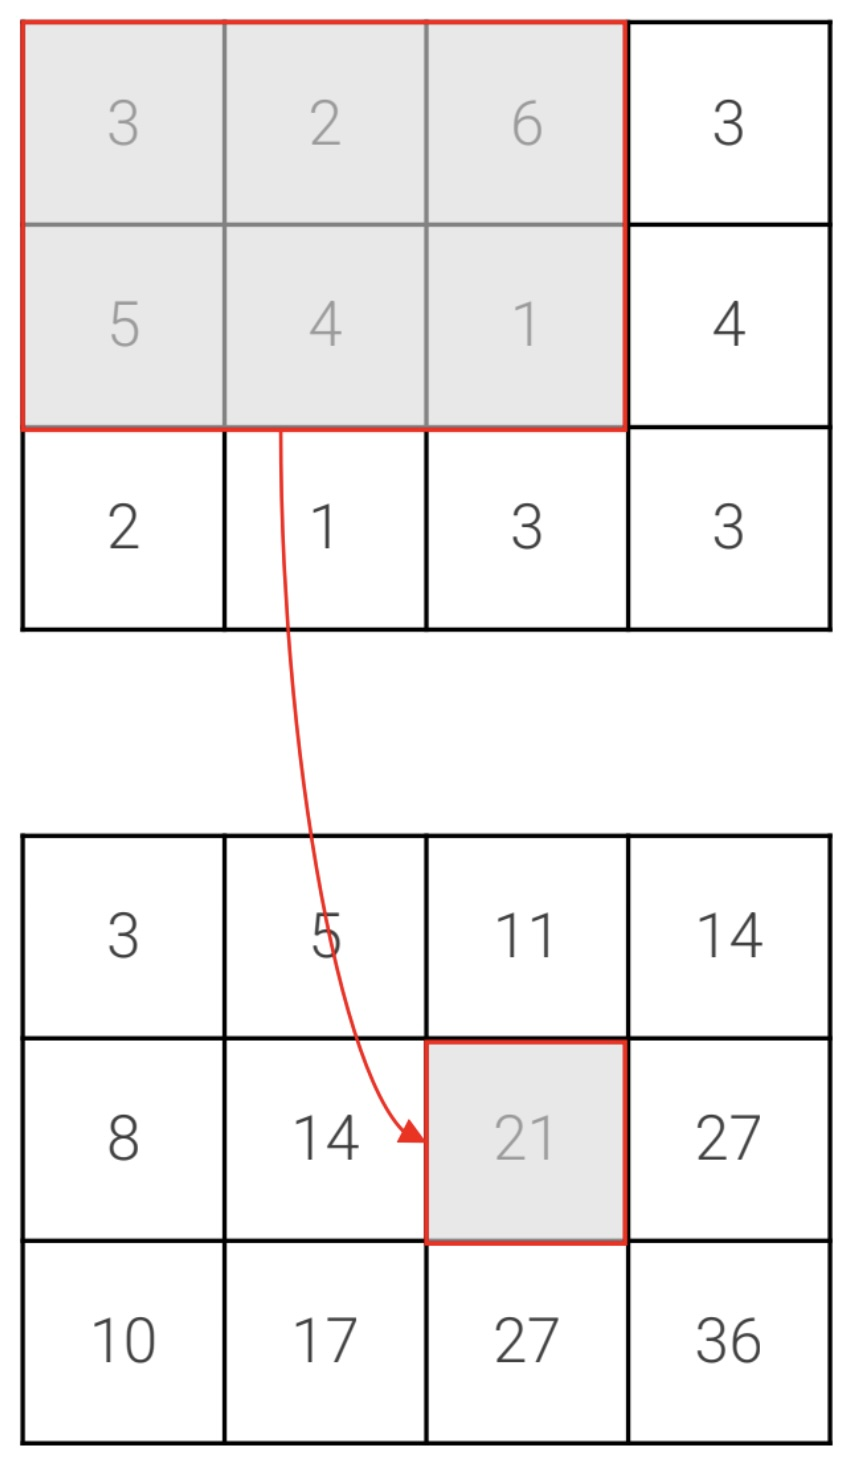
\includegraphics[width=0.3\linewidth]{./img/integral_images.jpg}
  \caption{$II(1,2) = II(1,1) + II(0,2) - II(0,1) + I(1,2) = 14 + 11 - 5 + 1$}
  \label{fig:integral_images}
\end{figure}

With integral images we could have an overflow problem if numbers get too big.
We can see an example of the calculation in the image \ref{fig:integral_images}

\begin{figure}[htbp]
  \centering
  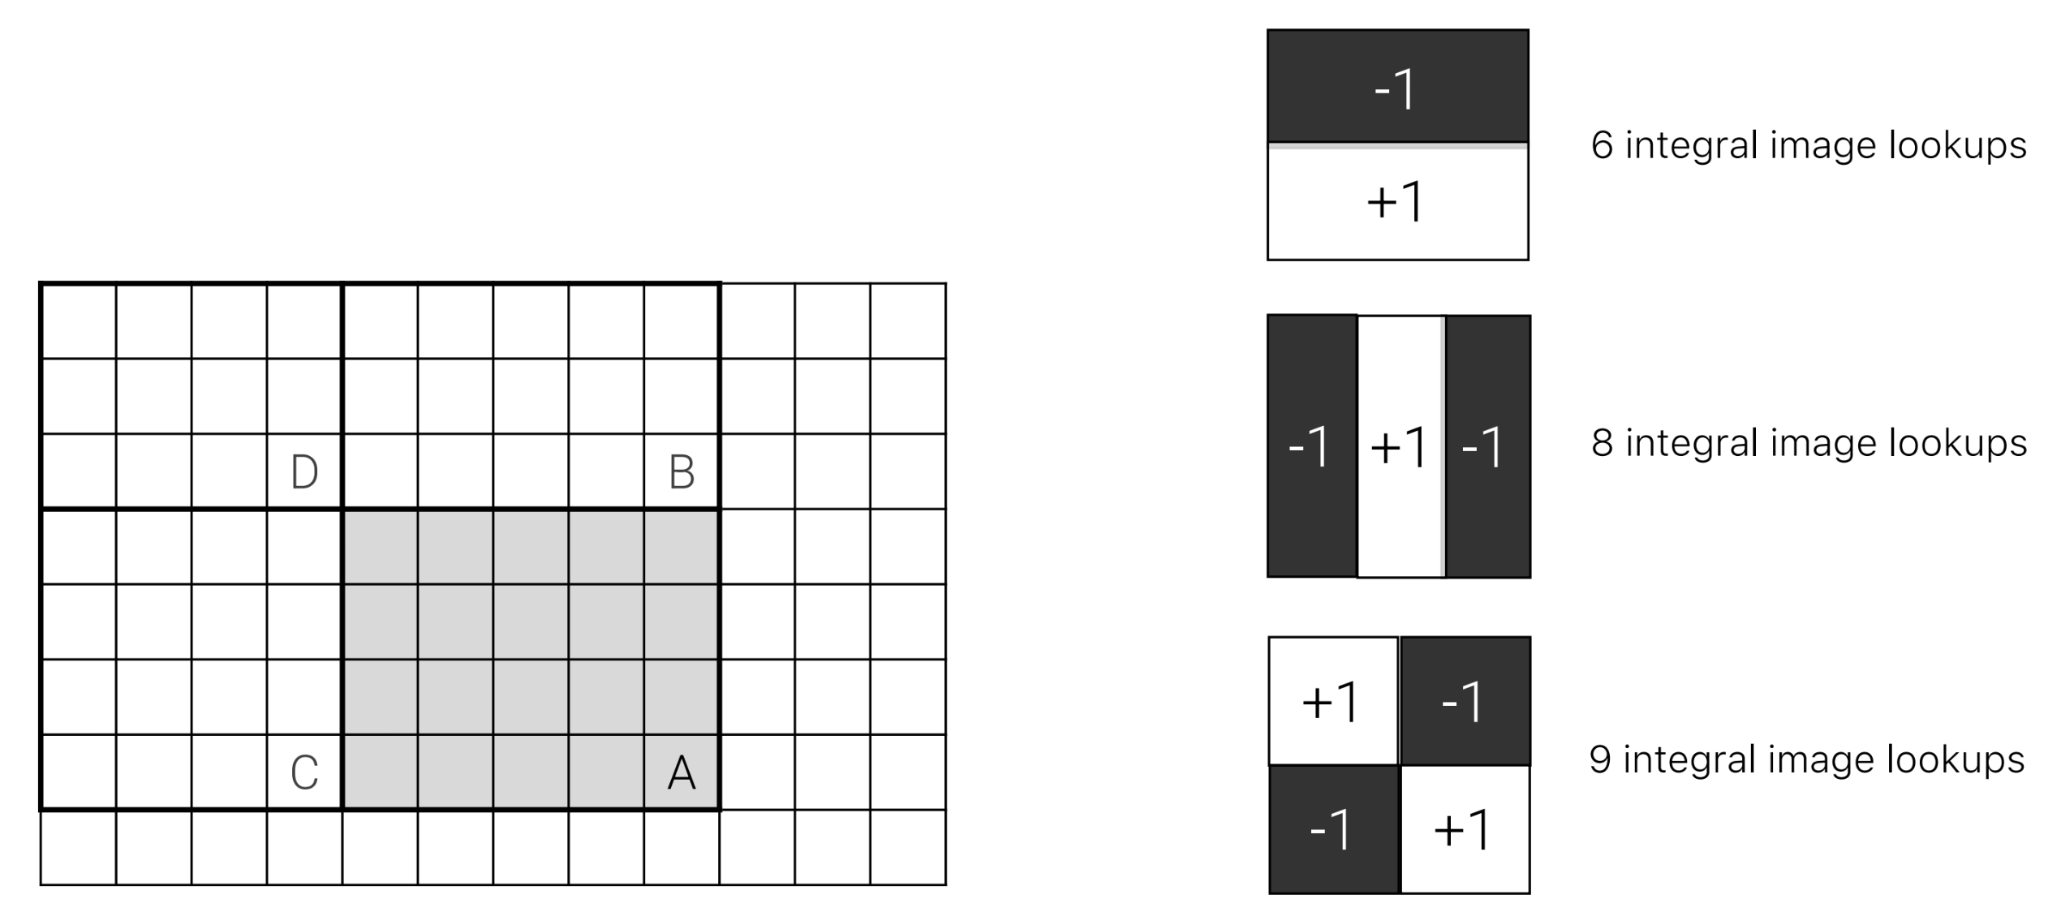
\includegraphics[width=0.6\linewidth]{./img/integral_filters.png}
  \caption{Rectangular filters can be computed in constant time with integral images}
\end{figure}

\paragraph{Multi-scale sliding window detector}
At test time, the strong classifier is applied to all spatial locations in the image.
Multi-scale detection is necessary, since faces are not necessarily $24\times 24$.
To achieve good performance, about 200 features are used to classify each patch.
Even if each feature can be computed very fast (thanks to integral images) there are still too many windows in an image to achieve real-time performance.

Faces are far less frequent in an image than background regions.
Most of the time is wasted computing a lot of features for background patches.
The key idea is then to reject most of the easy background patches with a simpler classifier which can be ran very fast.

\paragraph{Box overlap}

\begin{figure}[htbp]
  \centering
  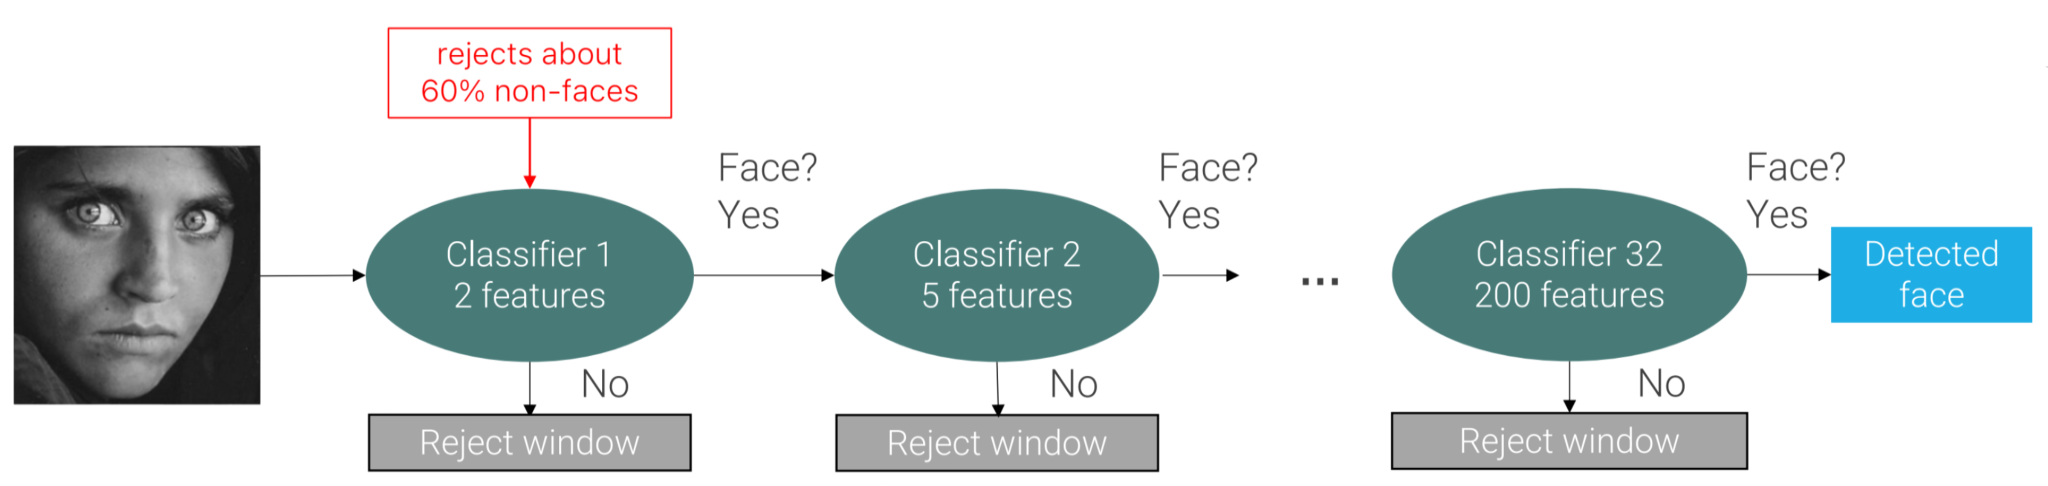
\includegraphics[width=0.8\linewidth]{./img/cascade_classifier.png}
  \caption{We use more and more features for face detection classifier after classifier}
\end{figure}

There will be several overlapping detections.
To check if two boxes overlap we measure the Intersection over Union ($IoU$) score: $IoU(BB_i, BB_j) = \frac{|BB_i \cap BB_j|}{|BB_i| + |BB_j| - |BB_i \cap BB_j|}$. $0.75$ corresponds to a good overlap, $0.90$ to a perfect one.
To obtain a single detection out of a set of overlapping boxes we perform Non Maxima Suppression of boxes.
Non Maxima Suppression considers the highest scoring Bounding Box, eliminates all the boxes with overlap greater than a threshold, and repeats this until all the boxes have been tested.

A detection is considered a True Positive if its overlap with the ground truth $BB^{GT}$ is greater than $\rho_{IoU}$.

\subsubsection{Transfer Learning}
If we can assume that only one object is present in the image, object detection simplifies to object localization.
Transfer learning is a technique where a model trained on one task is reused (or "transferred") for a different but related task.
Instead of training a model from scratch, you start with a pre-trained model and fine-tune it for your specific problem.
To solve object detection we can reuse any architecture used in image classification, by adding a regression head for predicting the bounding box.

We can apply a classification CNN as a sliding window detector.
We have to add a background class to discard background patches.
The problem is that there are too many boxes to try, since we have to try lots of positions with different scales and aspect ratios.
The solution is to use region proposals.

\subsubsection{Region proposals}
Region proposal algorithms inspect the image and attempt to find regions of an image that likely contain an object.
The algorithm as a first step oversegments the image into highly uniform regions, and then, \textbf{based on similarity scores of color, texture and size} it iteratively aggregates them.

\begin{figure}[htbp]
  \centering
  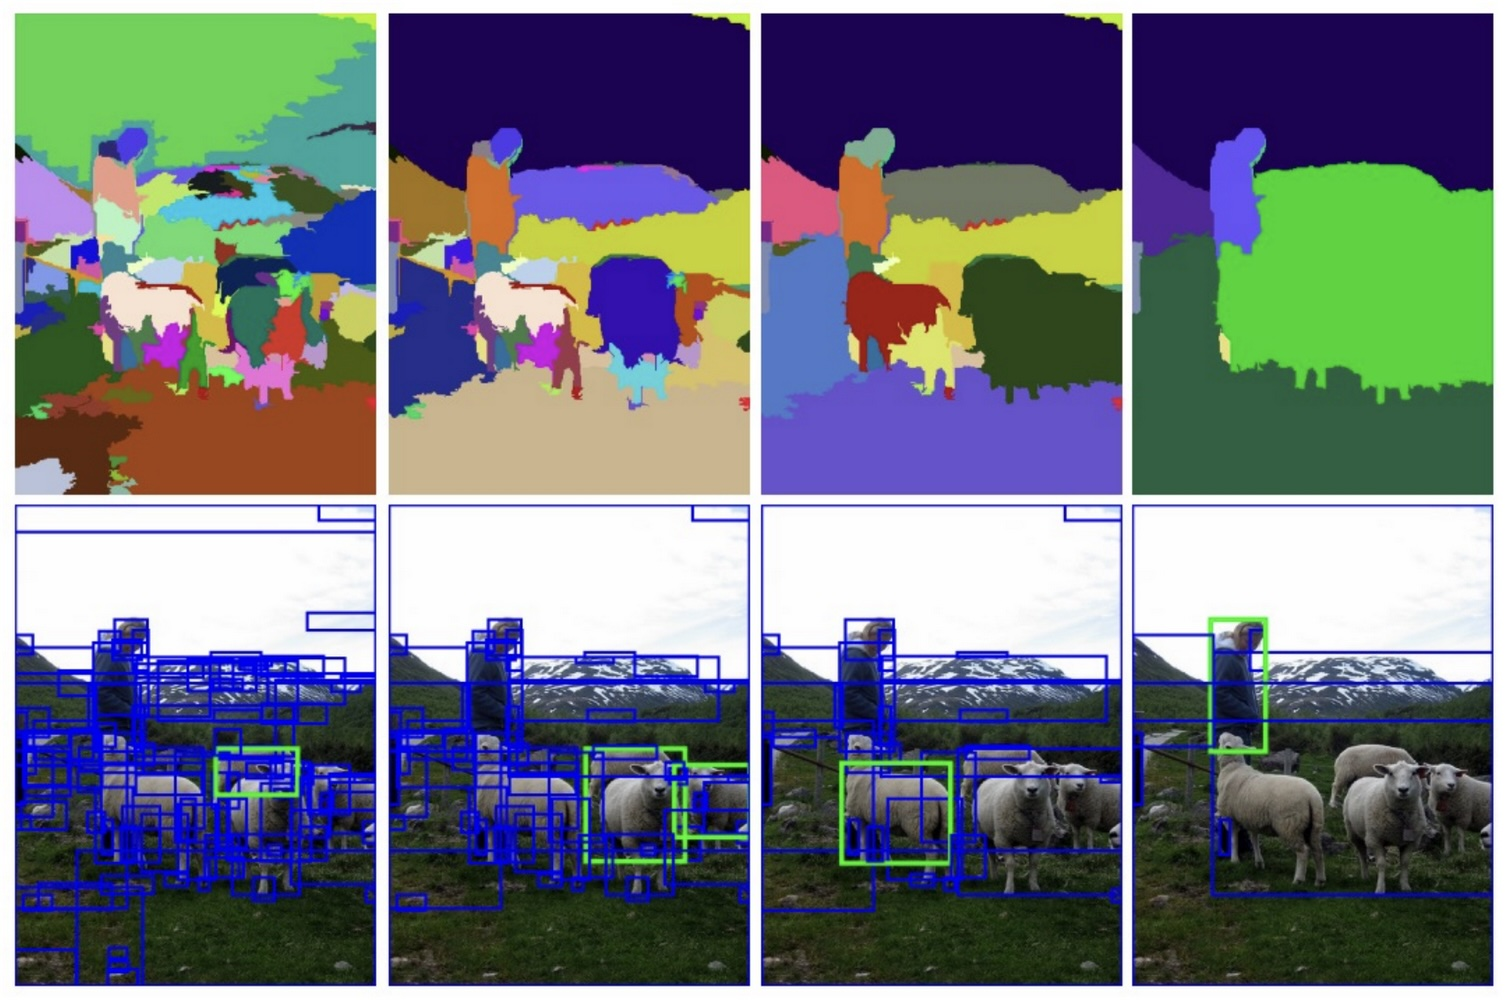
\includegraphics[width=0.6\linewidth]{./img/region_proposal.jpg}
  \caption{The 2 most similar regions are grouped together and then new similarities are calculated between the resulting region and its neighbors}
\end{figure}

\subsubsection{R-CNN: Region-based CNN}

Region-based CNN is the first object detector network.
As we can see in \ref{fig:rcnn} we run selective search to get about 2000 proposals, then we anisotropically (not uniformly across all directions) warp these proposals and add some pixels of context into a fixed size, to be able to input them in AlexNet, and for each proposal we get a class and a bounding box correction.

\begin{figure}[htbp]
  \centering
  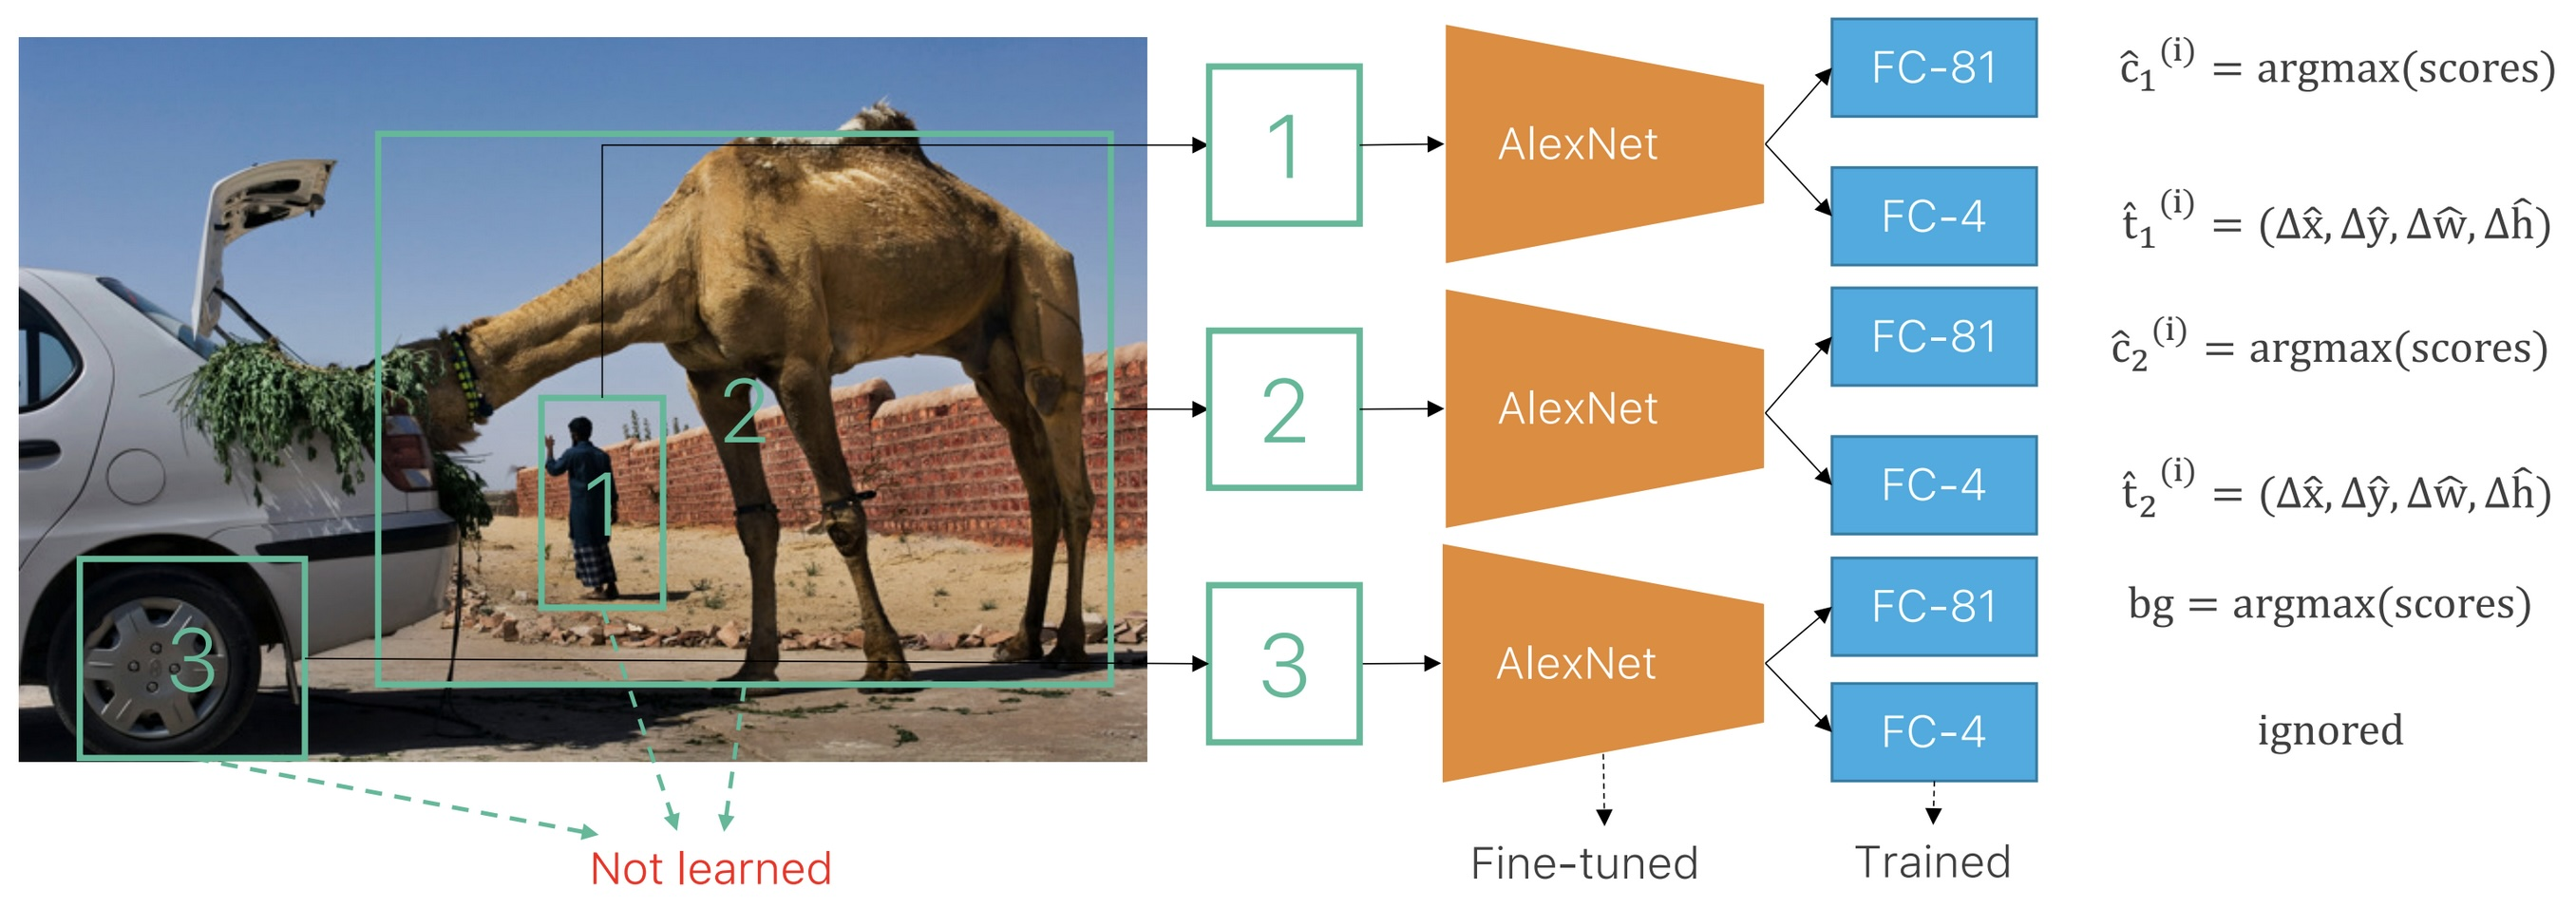
\includegraphics[width=0.8\linewidth]{./img/rcnn.jpg}
  \caption{R-CNN network architecture}
  \label{fig:rcnn}
\end{figure}

The problem is that since we have 2 different algorithms (one for the region proposal and one for AlexNet) we can't backpropagate through both of them.

\subsubsection{Fast R-CNN}

In the Fast R-CNN architecture showed in \ref{fig:fastrcnn} we can see that the model has been modified to run the first few layers of AlexNet on the original image, apply RoI pooling to crop and warp convolutional features according to proposal, and then run a small per-region network on each region to get the output class and bounding box correction.
This results in a faster networks since we don't have to apply 2000 CNN forward passes per image, but we apply most of the CNN before warping.

\begin{figure}[htbp]
  \centering
  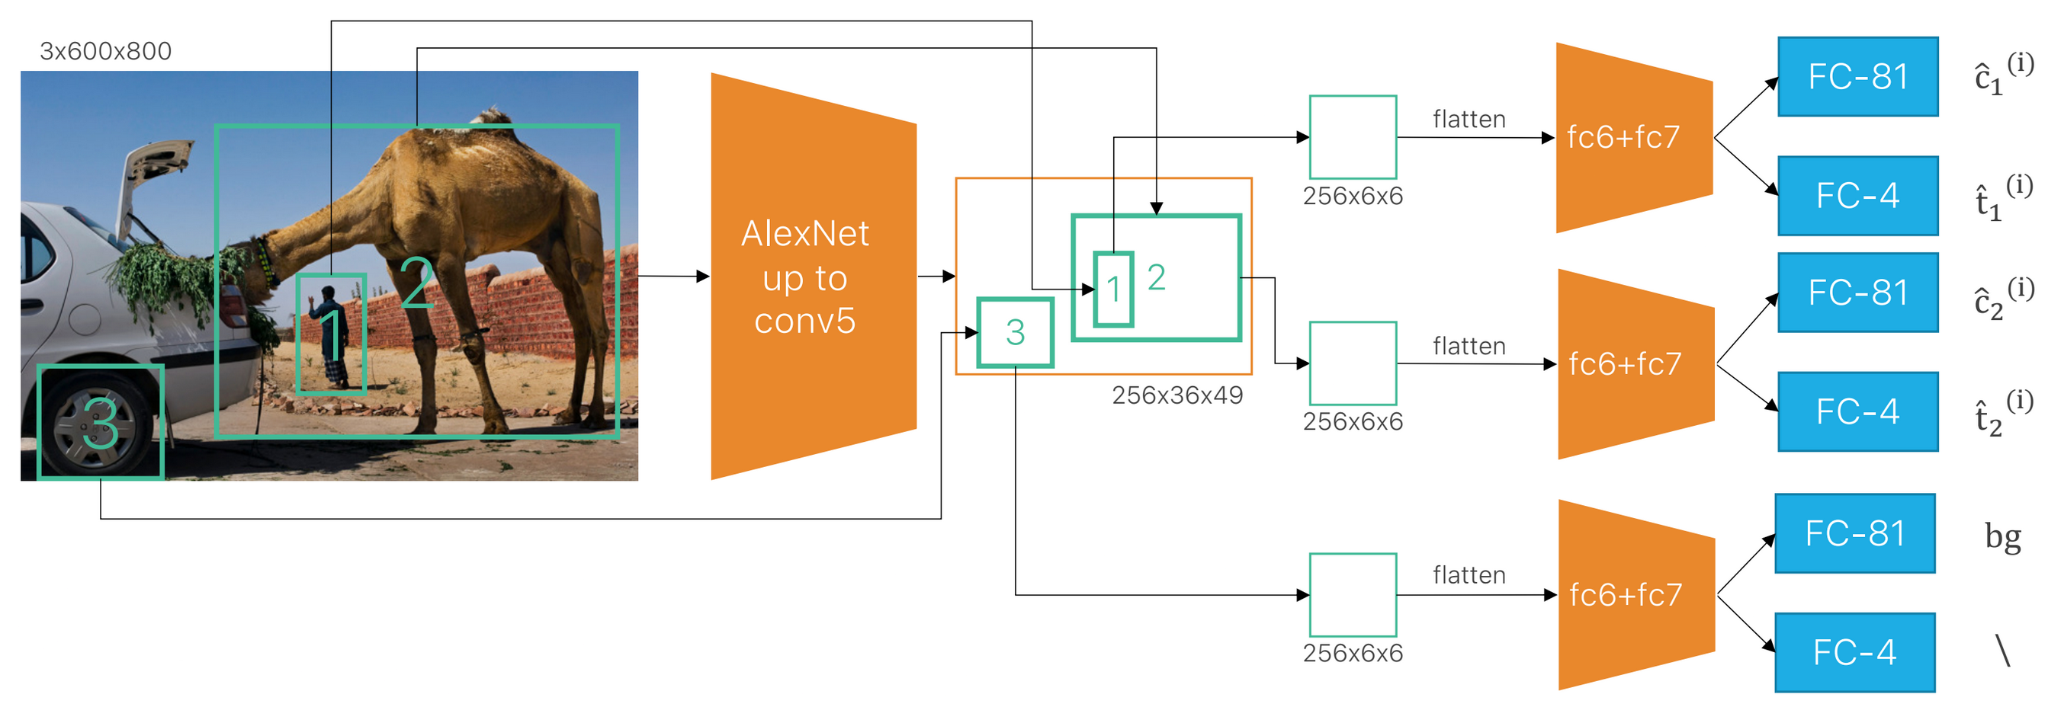
\includegraphics[width=0.8\linewidth]{./img/fastrcnn.png}
  \caption{Fast R-CNN network architecture}
  \label{fig:fastrcnn}
\end{figure}

Fast R-CNN uses the same bounding box correction of R-CNN, but with a smooth L1 loss (equal to L2 near the origin, but smoother elsewhere).

\paragraph{RoI pooling}
The RoIPool layer converts activations inside Region of Interest, corresponding to rescaled Selective Search regions, into activations with fixed spatial dimensions, which are the ones required by the remaining layers of the network.
To do RoI pooling, given a region:
\begin{enumerate}
  \item Snap the region to the grid.
  \item Apply max pooling kernels with approximate size $[H_r/H_o]\times [W_r/W_o]$ and approximate stride $s = [H_r/H_o]\times[W_r/W_o]$.
\end{enumerate}

\begin{figure}[htbp]
  \centering
  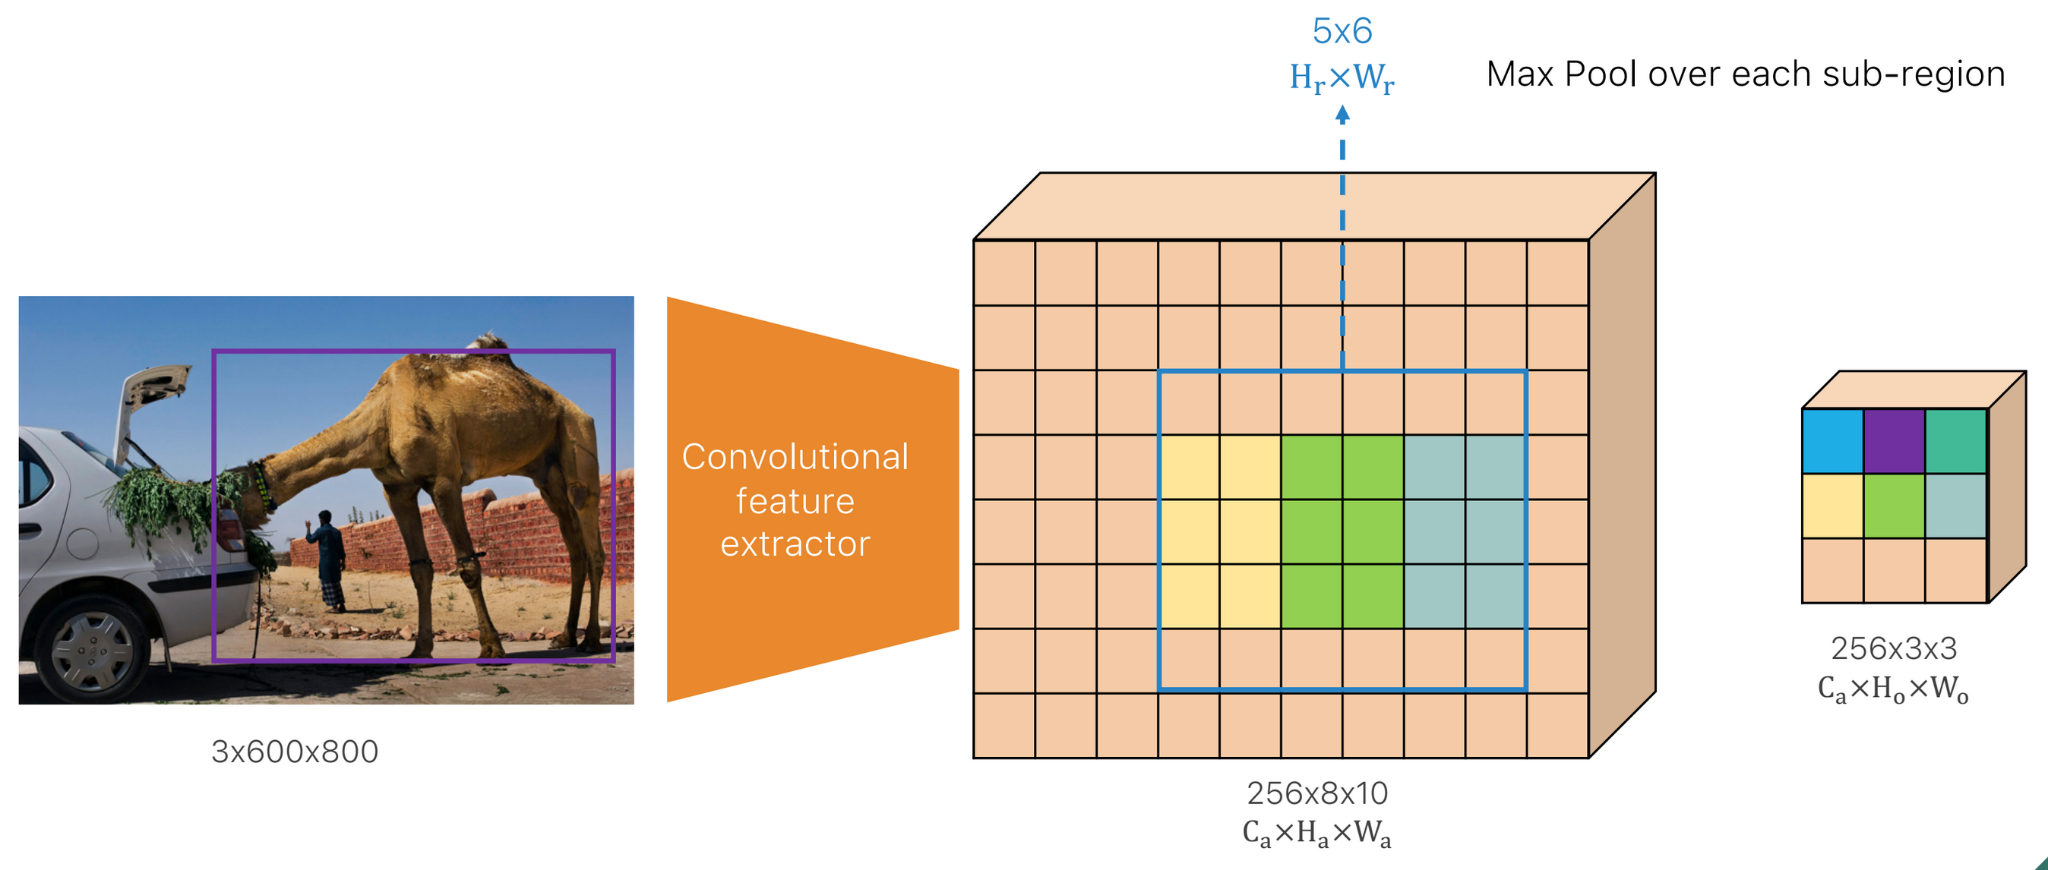
\includegraphics[width=0.7\linewidth]{./img/roipool.png}
  \caption{RoI pooling.}
\end{figure}

\subsubsection{Faster R-CNN}

In Fast R-CNN proposals are not learned, so the selective search is slow.
In Faster R-CNN they introduced a RPN (Region Proposal Network), which learns to predict the proposal box and the objectness score.

\begin{figure}[htbp]
  \centering
  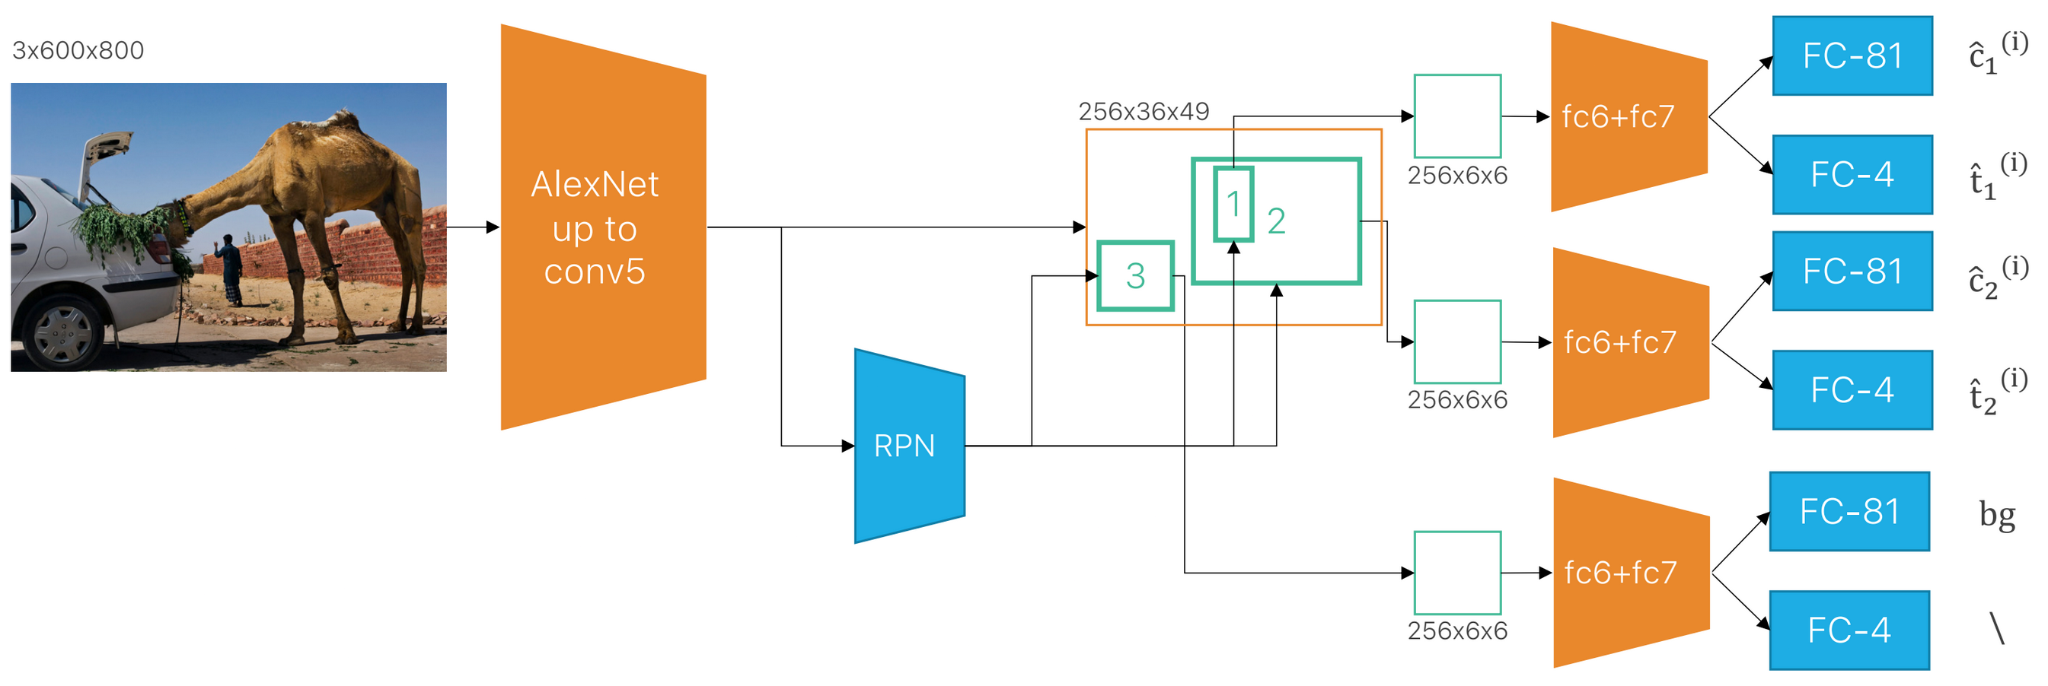
\includegraphics[width=0.8\linewidth]{./img/fasterrcnn.png}
  \caption{Faster R-CNN network architecture.}
\end{figure}

\paragraph{Region Proposal Network}

Region Proposal Networks are applied to a small $3\times 3$ window, which is approximately an object sized window in the original image and doesn't correspond to what we see in \ref{fig:rpn}, predicts the objectness and proposal bounding box.

\begin{figure}[htbp]
  \centering
  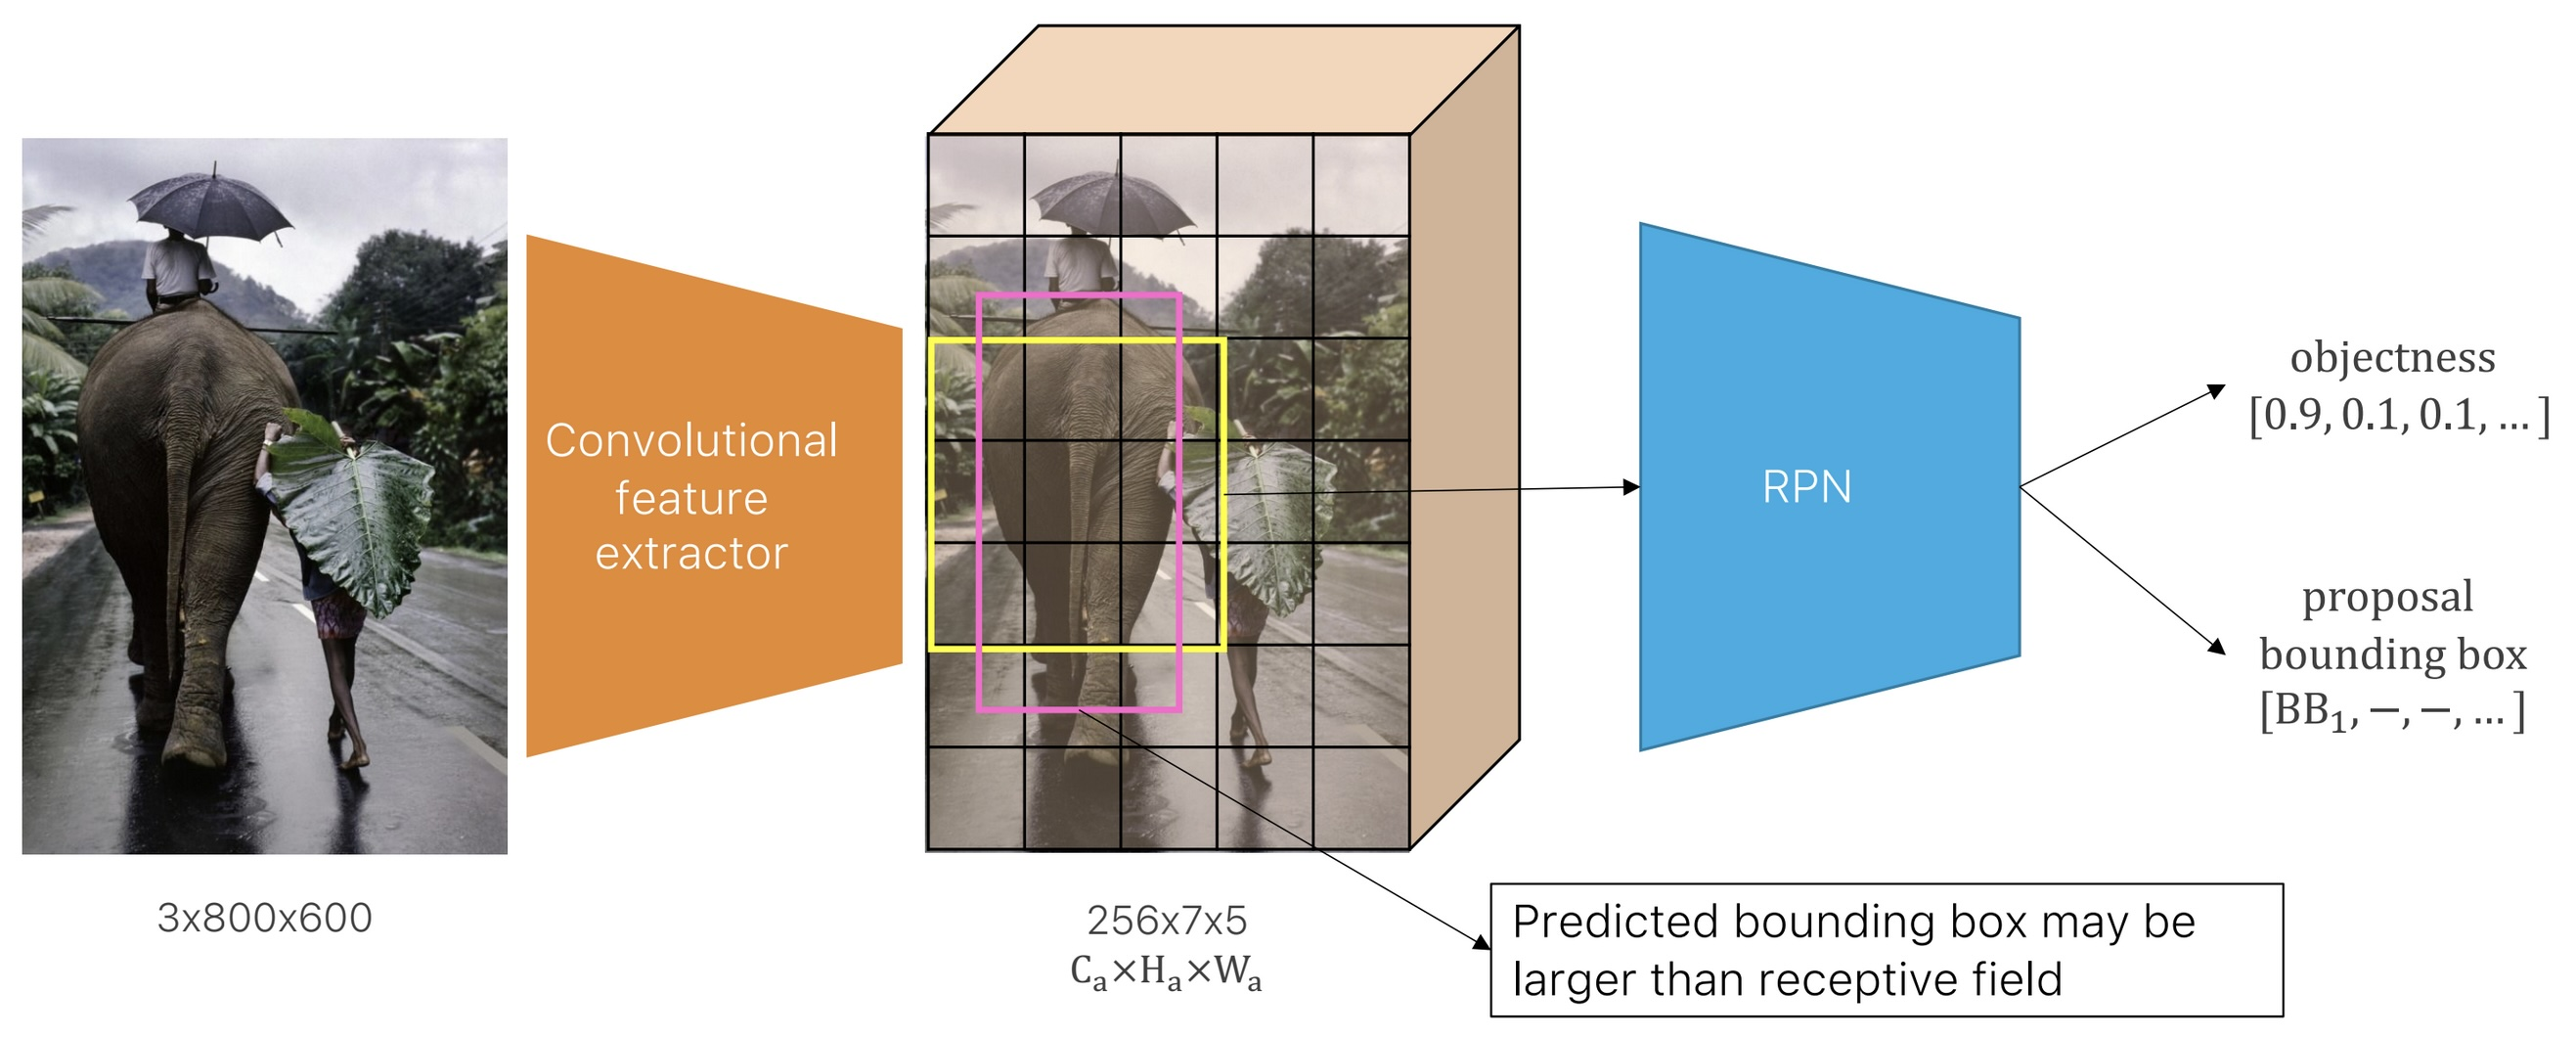
\includegraphics[width=0.7\linewidth]{./img/rpn.jpg}
  \caption{Region Proposal Network architecture.}
  \label{fig:rpn}
\end{figure}

When the objectness score is low, the localization head produces its output, but it's meaningless and it will be ignored.

\paragraph{Region Proposal Network with Anchors}
The process of generating object proposals can be simplified. Instead of predicting proposals from scratch, it is easier to refine a set of initial reference boxes, similar to the approach used in R-CNN.

\begin{figure}[htbp]
  \centering
  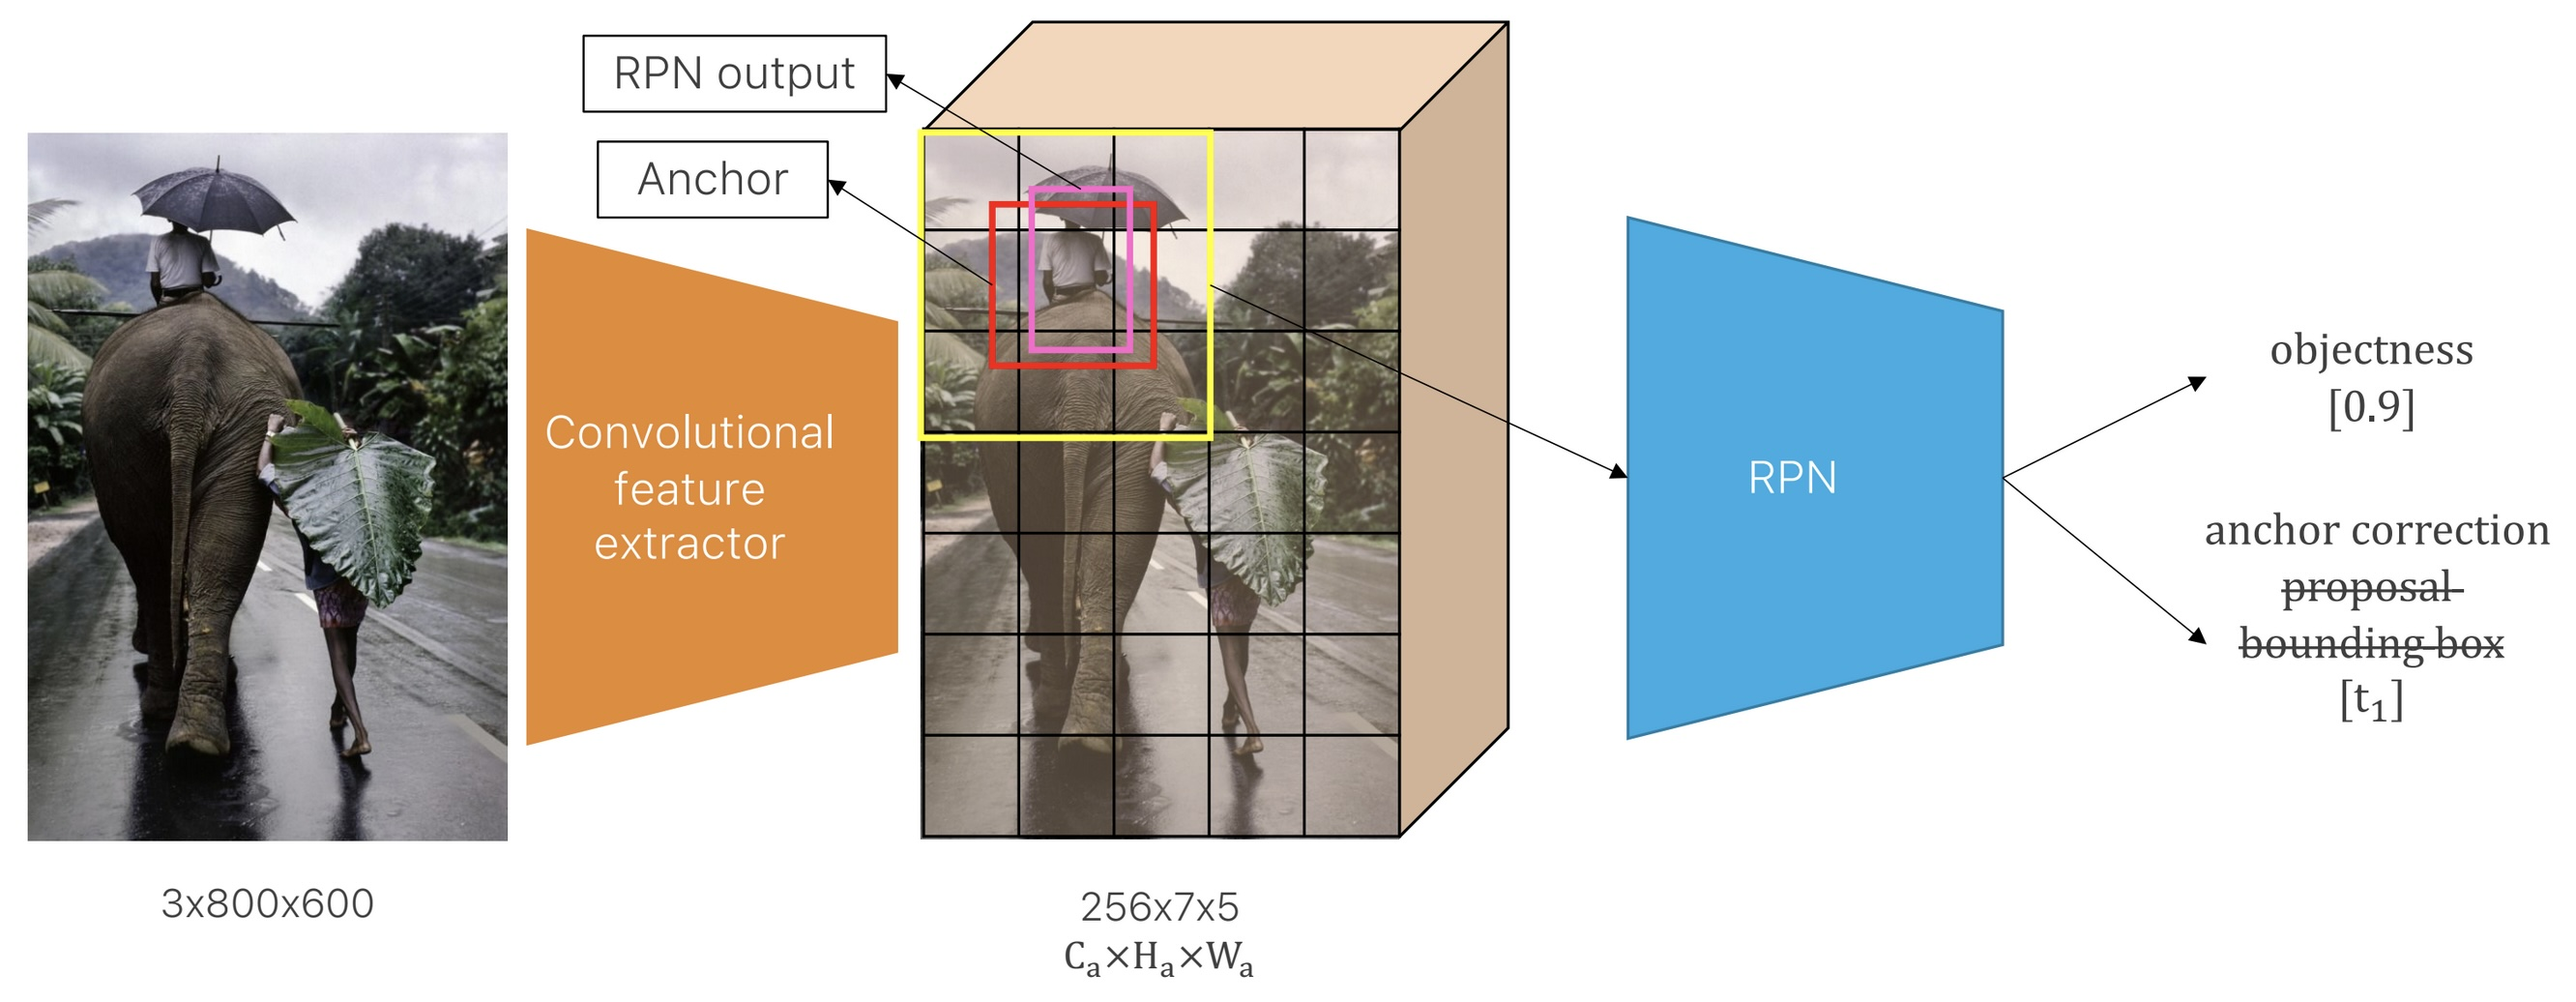
\includegraphics[width=0.6\linewidth]{./img/rpn_anchor.jpg}
  \caption{An anchor is a reference box with fixed scale and aspect ratio.}
\end{figure}

Since objects vary in scale and aspect ratio, we use multiple anchors at each spatial location, each with a different combination of scale and aspect ratio. The RPN predicts $k$ objectness scores and $k$ bounding box refinements for the $k$ anchors at each location.

During training, for a given image and its ground-truth bounding boxes, an anchor is labeled as background if it has low Intersection over Union (IoU) with all ground-truth boxes in the image.

In standard Faster R-CNN, the RPN operates on the final activation layer of the feature extractor. This feature map contains rich semantic information due to its depth in the network, but has low spatial resolution. As a result, even with small-scale anchors, \textbf{the RPN might fail to detect objects that are smaller than the grid size} of the feature map.

% slide 62/71
\subsubsection{Feature Pyramid Network (FPN)}
To do object detection at multiple scales, the naive approach is to obtain feature pyramids with CNNs, by running a CNN at each scale of the image, and then perform detection on each activation.
This is very bad for inference and training times.

A better approach is to give as input to the Region Proposal Network different stages of a CNN.
This is done because CNNs produce a pyramid of features, with different semantic qualities at different depths.
But different stages of a CNN have different input sizes (more channels as we go deeper in the network).

\begin{figure}[htbp]
  \centering
  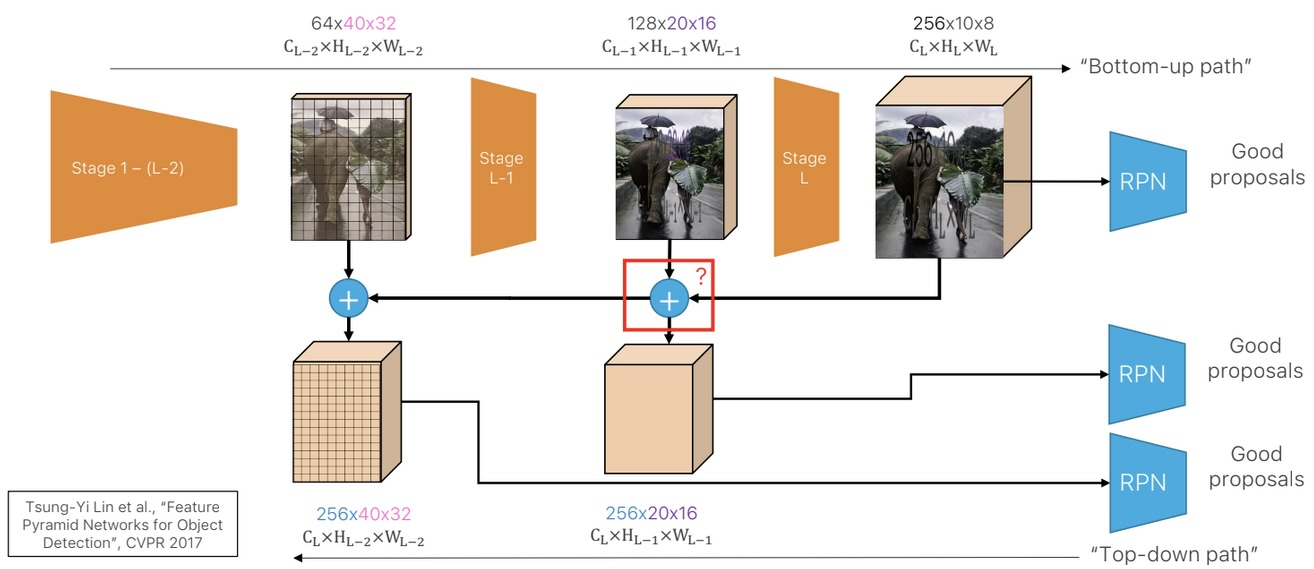
\includegraphics[width=0.7\linewidth]{./img/fpn.jpg}
  \caption{Feature Pyramid Network architecture.}
\end{figure}

Feature Pyramid Networks overcome this problem by merging coarser but higher level features with less effective but more spatially localized features.
This has a limited computational overhead.

\begin{figure}[htbp]
  \centering
  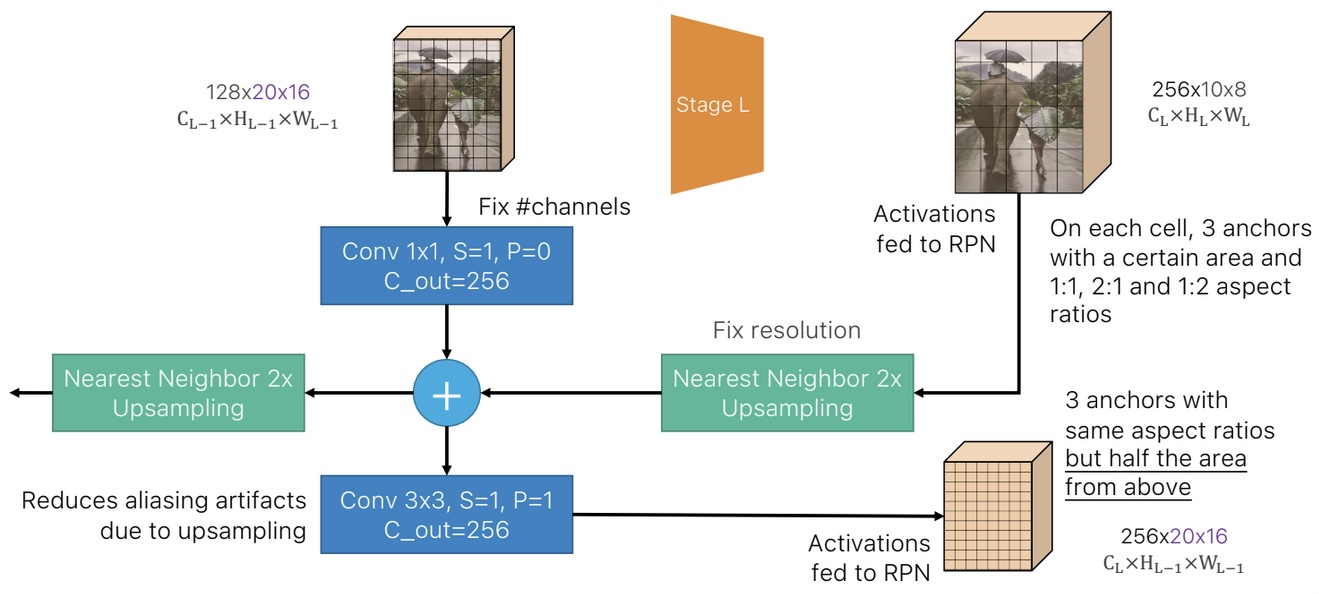
\includegraphics[width=0.7\linewidth]{./img/fpnsum.jpg}
  \caption{FPN top down path and lateral connections.}
  \label{fig:fpnsum}
\end{figure}

In \ref{fig:fpnsum} we can see how the FPN sums together different size pictures.
To fix the resolution we use Nearest Neighbor upsampling.
To fix the number of channels we use $1\times 1$ convolutions.

\subsubsection{Faster R-CNN with FPN}
We can use the FPN for the detection stage.
We use the FPN as a feature extractor which provides a pyramid of activations.
Then we can do the usual processing with the RPN and the per-region MLP.

\begin{figure}[htbp]
  \centering
  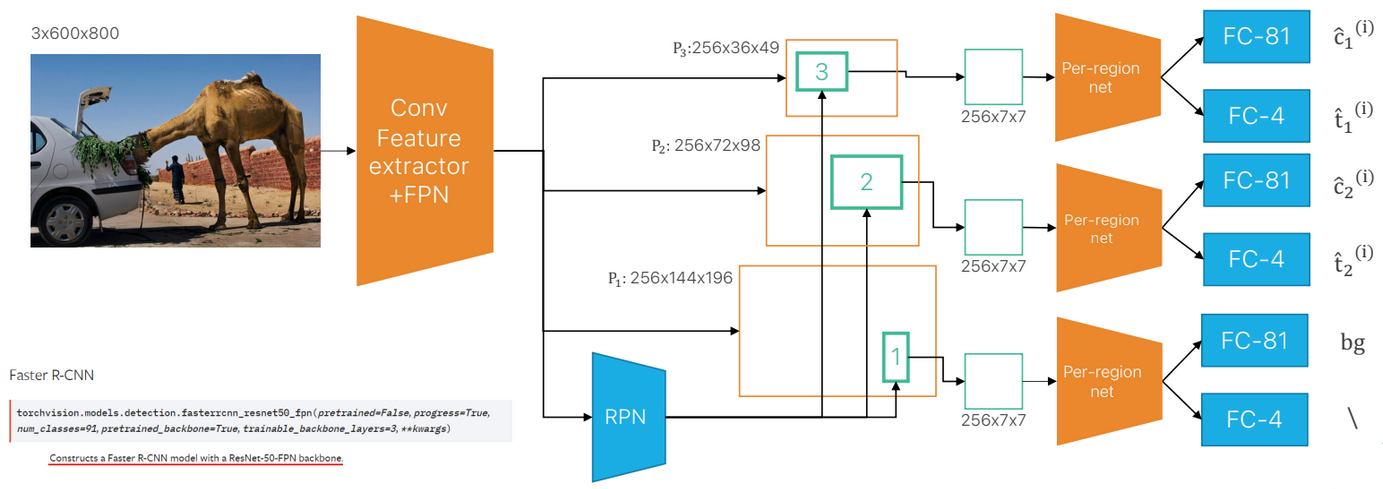
\includegraphics[width=0.8\linewidth]{./img/frcnn_fpn.png}
  \caption{Faster R-CNN with FPN architecture; as we can see we use the FPN together with the convolutional feature extractor.}
  \label{fig:frcnn_fpn}
\end{figure}

Introducing the FPN enables better model accuracy but gives no speedup, since we didn't change anything with the broader architecture.

\subsubsection{One Stage detectors}
As wee can see from the image \ref{fig:frcnn_fpn}, we have two main stages in the network architecture.
The first stage runs the expensive backbone feature extractor with the FPN on the full image, and the RPN generates the proposals for the bounding boxes.
This is done one time per each image.
The second stage, which is ran once per proposal, has a RoI pool, and a per-region classification and correction.

Instead of a RPN we could try to do all the job by using anchors, since the only things they are missing is learning the anchor dimensions and the class prediction.

\begin{figure}[htbp]
  \centering
  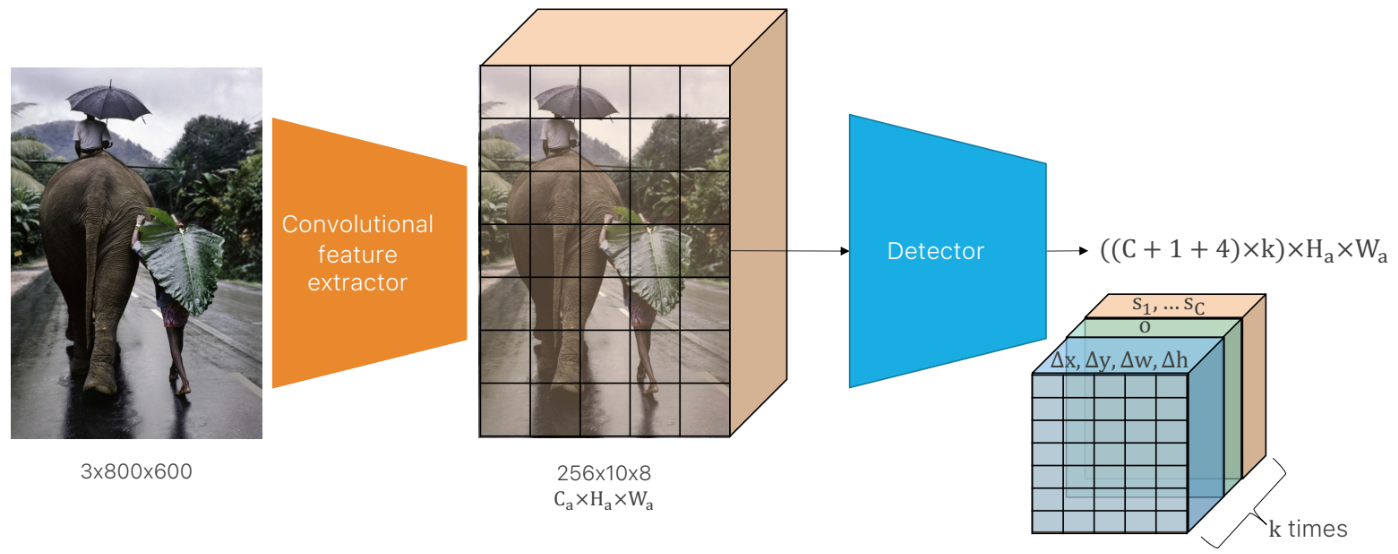
\includegraphics[width=0.8\linewidth]{./img/one_stage_detector.png}
  \caption{in one-stage detectors we can stack the outputs in a combined single tensor with the appropriate number of channels.}
\end{figure}

\subsubsection{SSD: Single Shot MultiBox Detector}

SSD applies multiple detection heads, implemented as $3 \times 3$ convolutions, across several feature maps. Each detector outputs $k_s \times (C + 1 + 4)$ channels, where $k_s$ is the number of anchors per location at that scale, $C$ is the number of classes, 1 accounts for the background class, and 4 corresponds to bounding box coordinates.

These detectors are applied both to intermediate feature maps from the backbone network (e.g., VGG) and to additional feature maps generated by stacking extra convolutional layers beyond the backbone.

\newpage
\begin{figure}[htbp]
  \centering
  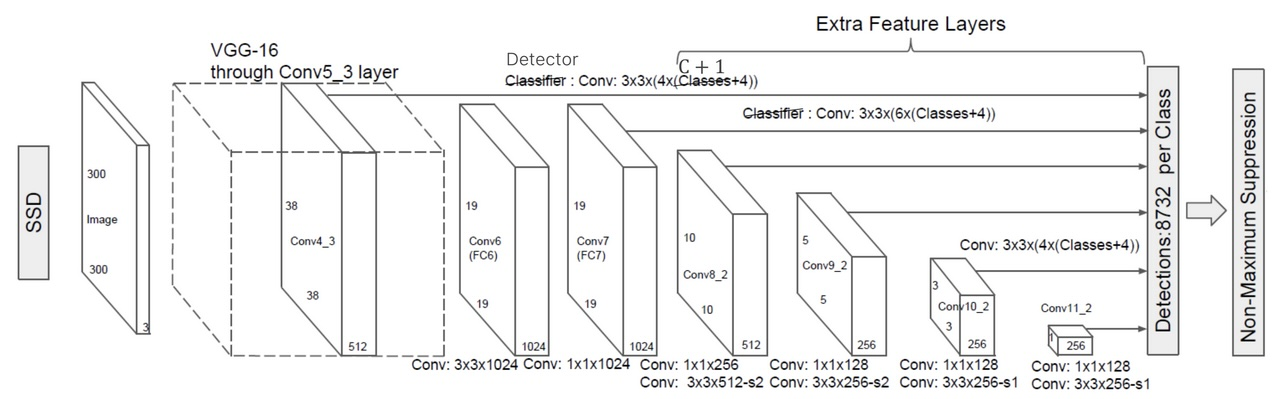
\includegraphics[width=0.9\linewidth]{./img/ssd.jpg}
  \caption{Single Shot MultiBox Detector architecture}
\end{figure}

\subsubsection{YOLOv3}

YOLOv3 employs a custom backbone called DarkNet-53, which balances classification accuracy and inference speed. It performs detections at multiple scales by concatenating feature maps from different stages, similar to an FPN (Feature Pyramid Network) but using concatenation instead of addition.

\begin{figure}[htbp]
  \centering
  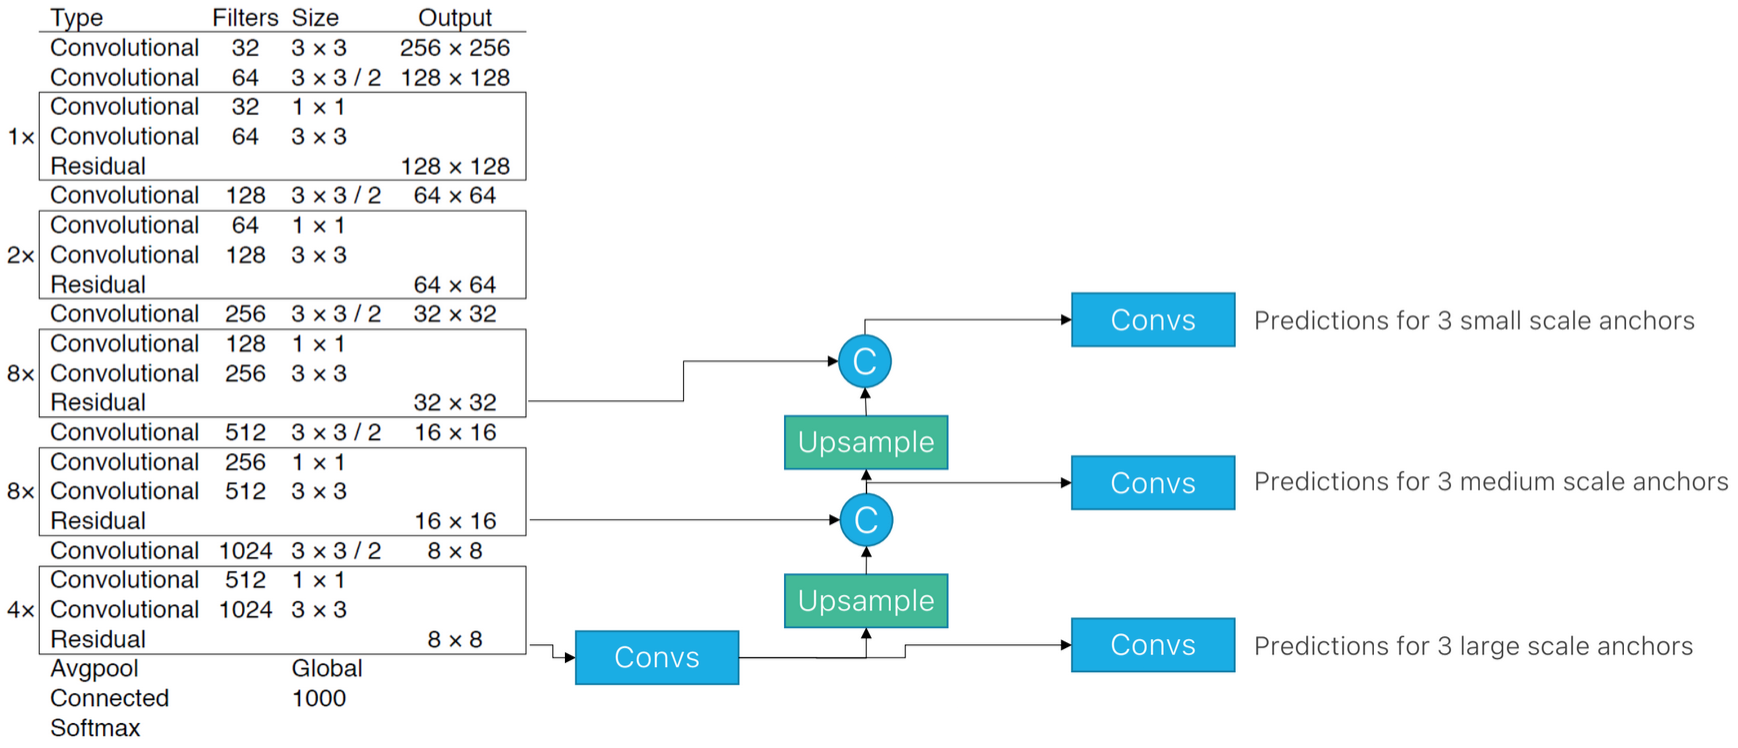
\includegraphics[width=0.9\linewidth]{./img/yolov3.png}
  \caption{YOLOv3 architecture}
\end{figure}

Anchor boxes (sizes and aspect ratios) are determined via k-means clustering on the ground-truth bounding boxes of the training dataset. By initializing predictions close to these clustered anchors, the network can converge more quickly. In practice, the resulting anchors tend to be similar across various datasets.

\subsubsection{RetinaNet}

RetinaNet is a one-stage detector built on top of a standard ResNet backbone with an integrated Feature Pyramid Network (FPN). It has separate classification and regression “heads,” each composed of stacked $3\times3$ convolutional layers. Unlike RPN (Region Proposal Network), these heads do not share parameters, since classification and bounding-box regression require different feature representations.

\begin{figure}[htbp]
  \centering
  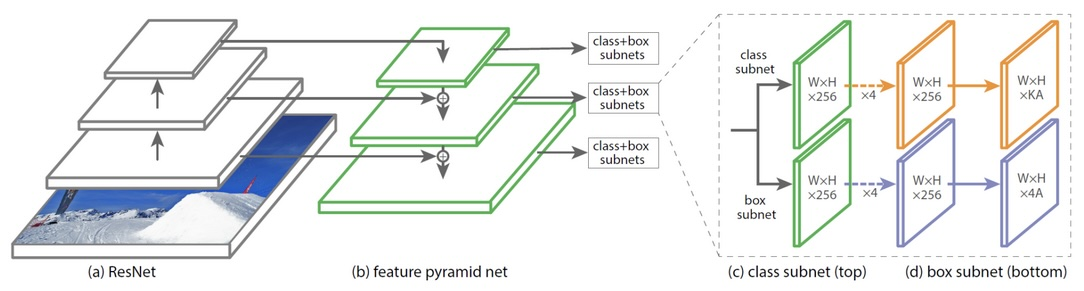
\includegraphics[width=0.9\linewidth]{./img/retina_net.jpg}
  \caption{RetinaNet architecture}
\end{figure}

\paragraph{The class-imbalance challenge}
In object detection, the number of negative (background) anchors far exceeds the number of positive (object) anchors. This imbalance causes two main issues:

\begin{enumerate}
  \item “Easy” negatives (anchors with low objectness scores) can dominate the loss, making it hard for the model to learn to discriminate between hard negatives and true positives.
  \item Most randomly sampled mini-batches will contain predominantly easy negatives, providing little useful gradient signal and slowing down training.
\end{enumerate}

Two-stage detectors mitigate this by sampling “hard” negatives: only high-scoring region proposals are passed to the second stage. By contrast, one-stage detectors must train on all anchors, including many easy negatives.

\paragraph{Focal loss}
To address this, RetinaNet uses focal loss, which down-weights easy examples and focuses training on hard examples. For a binary classification task, the standard cross-entropy (CE) loss is
\[
\mathcal{L}_{\text{CE}}(p, y) \;=\; -\bigl[y \ln(p) + (1 - y)\ln(1 - p)\bigr],
\]
where $p$ is the model's estimated probability that $y=1$. Defining 
\[
p_t = 
\begin{cases}
p, & \text{if } y = 1,\\
1 - p, & \text{if } y = 0,
\end{cases}
\]
we can write $\mathcal{L}_{\text{CE}}(p, y) = -\ln(p_t)$.

The focal loss introduces a modulating factor $(1 - p_t)^\gamma$:
\[
\mathcal{L}_{\text{FL}}(p_t) \;=\; -(1 - p_t)^\gamma \ln(p_t),
\]
where $\gamma \ge 0$ is a focusing parameter (commonly $\gamma=2$). When $p_t$ is large (an “easy” example), $(1 - p_t)^\gamma$ becomes small, reducing the loss. For example:
\begin{itemize}
  \item If $p_t = 0.9$, then $(1 - p_t)^\gamma = (0.1)^2 = 0.01$, so the focal loss is 100$\times $ smaller than the CE loss.
  \item If $p_t = 0.6$, then $(1 - p_t)^\gamma = (0.4)^2 = 0.16$.
  \item If $p_t = 0.1$, then $(1 - p_t)^\gamma = (0.9)^2 = 0.81$, making the focal loss close to the CE loss.
\end{itemize}

\paragraph{Class weighting}
In addition to focal loss, RetinaNet applies standard class weights to balance the relative importance of positive and negative examples. Class weights ensure that errors on the minority class (foreground) receive higher weight, while focal loss focuses learning on hard examples within each class. Combining both mechanisms yields more stable and effective training.

\subsubsection{Key differences between YOLOv3 and RetinaNet}

\begin{itemize}
  \item \textbf{Backbone and feature fusion}:
    \begin{itemize}
      \item YOLOv3 uses DarkNet-53 and concatenates feature maps from different stages for multi-scale predictions.
      \item RetinaNet uses ResNet with an explicit FPN, which sums feature maps across levels and applies separate heads at each pyramid level.
    \end{itemize}
  \item \textbf{Detection heads}:
    \begin{itemize}
      \item YOLOv3 predicts boxes and class scores on a grid of three scales directly from concatenated features.
      \item RetinaNet has separate stacks of convolutional layers for classification and regression on each FPN level.
    \end{itemize}
  \item \textbf{Loss functions}:
    \begin{itemize}
      \item YOLOv3 uses binary cross-entropy (BCE) for classification and mean squared error (or IoU-based loss) for bounding-box regression.
      \item RetinaNet uses focal loss for classification (to address class imbalance) and smooth $L_1$ loss for bounding-box regression.
    \end{itemize}
  \item \textbf{Anchor initialization}:
    \begin{itemize}
      \item YOLOv3 learns anchoring by running k-means clustering on ground-truth boxes of the dataset.
      \item RetinaNet uses a fixed set of anchors defined by scale and aspect ratio at each FPN level (often chosen based on prior knowledge).
    \end{itemize}
\end{itemize}

\subsubsection{Multi-label classification}

In YOLOv3, class prediction for each bounding box is treated as a multi-label classification task, rather than a multi-class one: a single box can be assigned one or more of the $C$ classes, which are not assumed to be mutually exclusive.

As a result, YOLOv3 does not apply a softmax function to produce a single probability distribution over classes. Instead, it uses $C$ independent sigmoid activations—one per class—to estimate the probability that the box belongs to each class individually.

The classification loss for each box is then the sum of $C$ binary cross-entropy losses, one for each class.

Because the background is implicitly represented by a ground-truth vector of all zeros, there is no need to explicitly introduce a background class. At inference time, a box is considered background if all class scores fall below the detection threshold.

\subsubsection{CenterNet}
Anchors-based detectors, either two or one stage ones, have some limits:
\begin{itemize}
  \item Anchors are a brute force approach to detection: we are enumerating a subset of all possible boxes, which is very inefficient.
  Moreover, the more anchors the better, but it's not clear what the best way to use a subset is.
  \item We obtain a lot of duplicated entries for an object, which must be post-processed with NMS, so the detector is in practice not end-to-end differentiable.
  \item Assignment of anchors to ground truths for training is based on manually selected thresholds and hand-crafted rules.
\end{itemize}

To overcome these limits, CenterNet proposed to represent objects as points (which is also the name of the paper which introduced the network), and regress their size or other properties.
It's like the keypoints in Difference of Gaussians, but at a higher level, since the keypoints should be the center of my object.

Given an image of size $3 \times H \times W$, the aim of the network is to produce a heatmap $\hat{Y}$ with values $\in [0,1]$ and size $C \times \frac{H}{R} \times \frac{W}{R}$ with output stride $R$.
To recover the discretization error caused by the output stride, the network also predicts an offset for each center point.
Finally, it also predicts the bounding box size $\hat{S}$ of size $2 \times \frac{H}{R} \times \frac{W}{R}$.

The backbone used to produce the convolutional features are fully convolutional encoder-decoder architectures devised for keypoint detection or semantic segmentation.
All the 3 outputs are predicted from the last activation with a dedicated head.

Each ground truth keypoint (object center) $p = (x_p, y_p)$ of class $c$, is projected in the lower-resolution output heatmap $\tilde{p} = \lfloor \frac{p}{R} \rfloor$.
Then, the target heatmap for its class $Y_C$ is set to 1 at $\tilde{p}$ and updated with an unnormalized Gaussian kernel.
Points can be seen as a special case of anchor: a single, shape-agnostic, anchor.
Detection is performed by finding local maxima in a heatmap, with one box per object (so without using NMS), and based solely on location, not box overlap.

\begin{figure}[htbp]
  \centering
  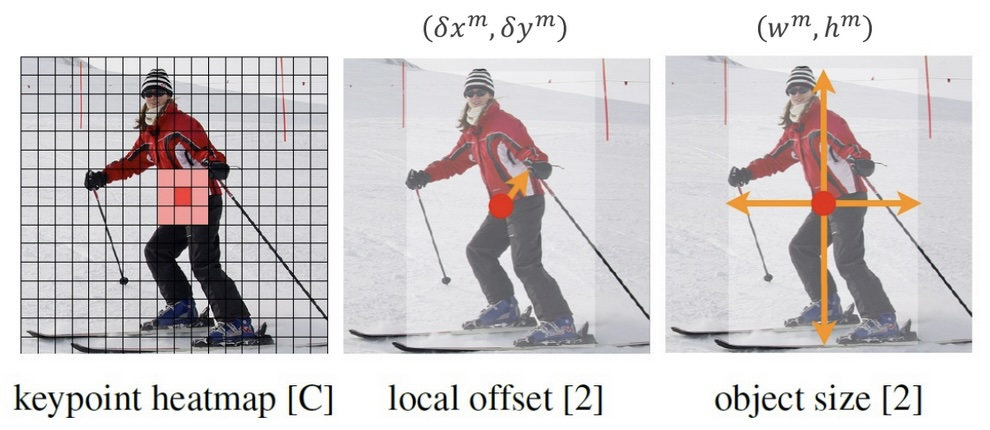
\includegraphics[width=0.9\linewidth]{./img/centernet.jpg}
  \caption{At inference time, given a spatial local maxima in the channel $\hat{Y_C}$ at position $(x^m, y^m)$, the box centered at $(x^m + \delta x^m, x^m + \delta y^m)$ of size $(w^m, h^m)$ and class $c$ is detected, without any further post-processing.}
\end{figure}


\subsection{Image segmentation}
In image segmentation we need to do per-pixel labelling, which is a costly task, since the input is the RGB image of size $W\times H$ and the output is \textbf{a category $c_{uv}$ for each pixel $p=(u,v)$}.
With $c_{u,v} \in [1,... ,C]$ which is a fixed list of categories.

\begin{figure}[htbp]
  \centering
  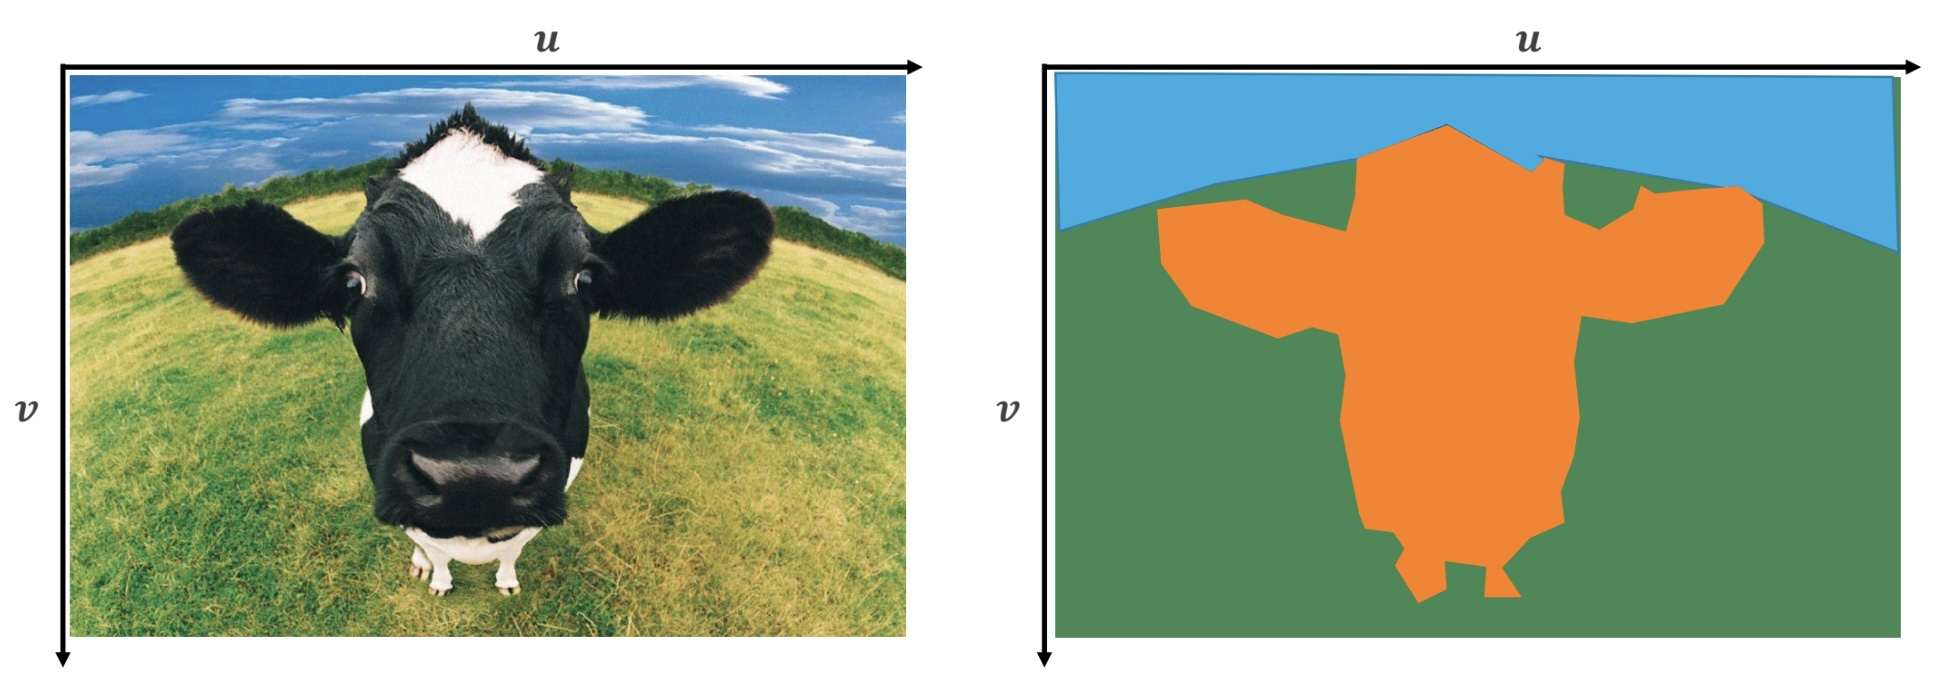
\includegraphics[width=0.7\linewidth]{./img/segmentation_task.jpg}
  \caption{On the right there is the output of the image segmentation task}
\end{figure}

We can try to use synthetic data to harvest the labels, i.e. with a videogame engine, where we exactly know what the objects are and where they are on the screen.
But this has the problem of domain shift (we can't learn to do segmentation on GTA V and then try to apply the same network on the real world).

\subsubsection{Generalized IoU and other measures}
The intersection over union can be generalized to segmentation masks by counting the pixels.
For a class $c = 1, ..., C$ we can define the Intersection over Union for the class as $IoU_C = \frac{\text{area of intersection}}{\text{area of union}}$.
To compute the mean IoU score for a dataset, we average $IoU_C$ over classes.
$mIoU = \frac{1}{C} \sum_{C=1}^{C} IoU_C$.

The $mIoU$ is the main measure to rank semantic segmentation algorithms.
Other measures are:
\begin{itemize}
  \item Pixel accuracy: the fraction of pixels correctly classified $\frac{\sum_{C} TP_C}{\text{\# pixels in the dataset}}$. This has the problem of being biased towards the largest object.
  \item Mean accuracy: the average of the accuracy for each class $\frac{1}{C} \sum_{C} \frac{TP_C}{\text{\# pixels of class }C \text{ in the dataset}}$.
  \item Frequency weighted IoU: weighted average of $IoU_C$ for each class, with weights given by the frequency of a class in the dataset $\sum_{C} \frac{\text{\# pixels of class }C}{\text{\# pixels in the dataset}} IoU_C$.
\end{itemize}

\subsubsection{Slow R-CNN for segmentation}
We can apply the same ideas used in R-CNN: we slide the window at all possible positions.
There are no proposals, since we must process each pixel, which is even slower than R-CNN for detection.

\begin{figure}[htbp]
  \centering
  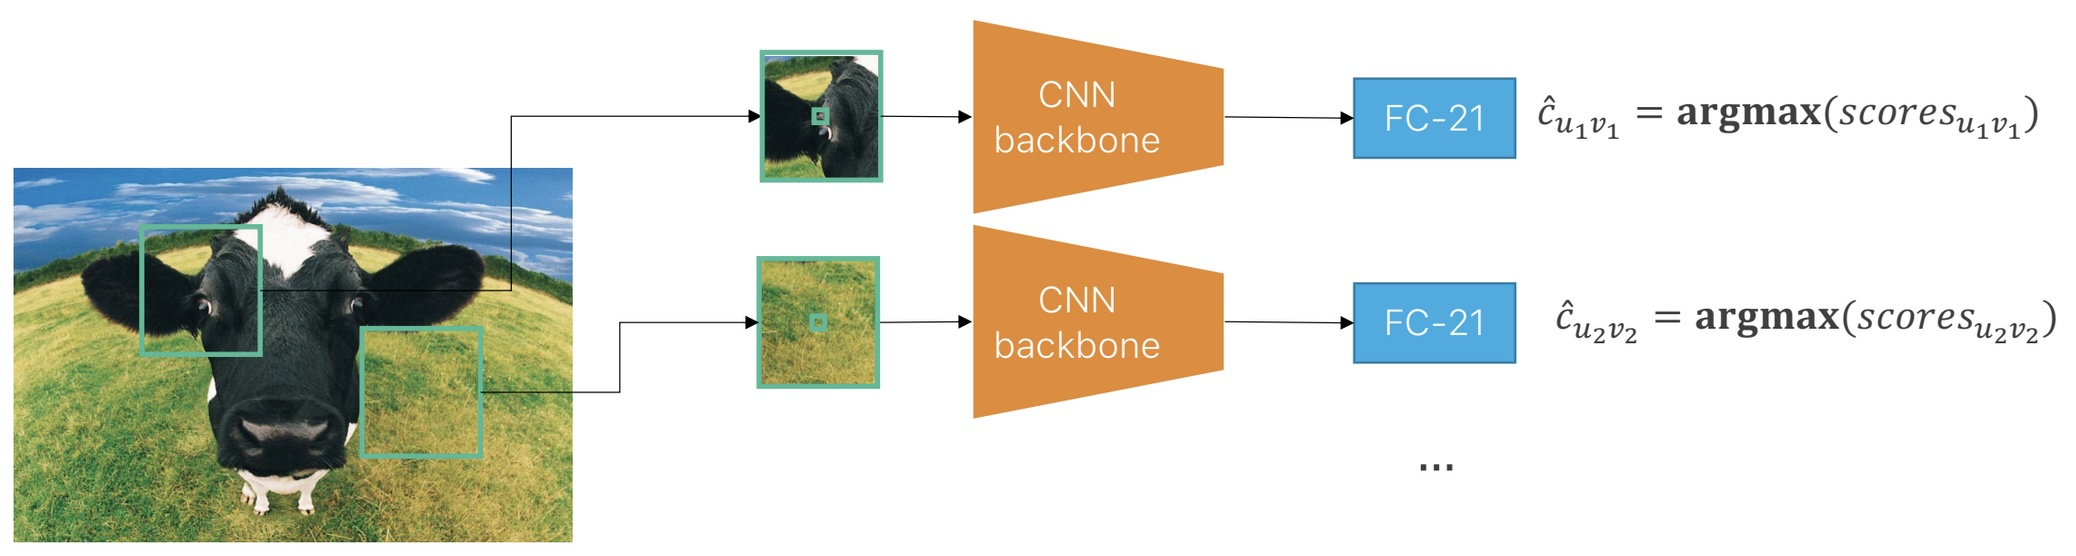
\includegraphics[width=0.8\linewidth]{./img/slow_rcnn_segmentation.jpg}
  \caption{Network architecture for Slow R-CNN for segmentation}
\end{figure}

As the loss we use the sum of the standard multi-class loss over all pixels:
$$L(\theta, x^{(i)}, y^{(i)}) = \sum_{u,v} CE\left(\text{softmax}(scores_{u,v}), \mathbf{1}(c_{u,v})\right)$$
With $\mathbf{1}$ which is the one-hot encoded ground truth class label for the pixel $(u,v)$.

The idea is that, as we did for detection, we can use a convolutional feature extractor and process the image through a CNN to get some activations and from that compute our output.
We have to go from the activations of the extractor to an output that has as many channels as the number of classes and the same resolution as the input.

\begin{figure}[htbp]
  \centering
  \includegraphics[width=0.7\linewidth]{./img/fcn_segmentation.jpg}
  \caption{We have to go from 512 channels to 21 channels with a $1\times 1$ conv. We have to go from a resolution of $6 \times 8$ to the original resolution of $256 \times 320$.}
\end{figure}

One way to perform the upsampling can be to use standard, not-learned, image processing operators (like bilinear interpolation).

\subsubsection{FCN-32s}
The FCN-32s (Fully Convolutional Network) is built on top of a CNN backbone.
It uses the deepest feature map of the CNN, and then applies a $1\times 1$ convolution to reduce the number of channels to the number of classes.
Then the network uses a single upsampling step by a factor of 32 (hence the name 32s) to bring it back to the input image size.

\begin{figure}[htbp]
  \centering
  \includegraphics[width=0.8\linewidth]{./img/fcn32.jpg}
  \caption{Network architecture for FCN-32s}
\end{figure}

The problem is that without learning a non-linear upsampling transformation, we can only uniformly spread the coarse information in the final convolutional activation, obtaining very coarse masks.
The solution is to upsample multiple activations at different resolutions (like with FPN).

\subsubsection{FCN-16s}
The FCN-16s adds additional connections between the output and the internal layers, which are referred to as skips.
This results to better spatial detail, with more accurate segmentation than FCN-32s.

\begin{figure}[htbp]
  \centering
  \includegraphics[width=0.8\linewidth]{./img/fcn16.png}
  \caption{Network architecture for FCN-16s}
\end{figure}

\subsubsection{FCN-8s}
In the FCN-8s we can consider one more intermediate layer (2 skip connections) with respect to the FCN-16s.

\begin{figure}[htbp]
  \centering
  \includegraphics[width=0.7\linewidth]{./img/fcn8.png}
  \caption{Network architecture for FCN-8s}
\end{figure}

With the VGG backbone, no more improvements were found after predicting from stride 8 activations (2 skip connections).

\subsubsection{Transposed Convolutions}

Standard convolutions with stride \(s>1\) perform learnable downsampling by skipping \(s-1\) input positions between successive kernel applications. To invert this process and learn upsampling, we can use \emph{transposed convolutions}, sometimes also called \emph{fractionally strided convolutions} or \emph{upconvolutions}.

\begin{figure}[htbp]
  \centering
  \includegraphics[width=0.7\linewidth]{./img/fractional_conv.png}
  \caption{Inserting zeros between input pixels (fractional stride) yields a larger feature map before convolution.}
  \label{fig:fractional_conv}
\end{figure}

Conceptually, one can imagine upsampling by first “expanding” the input: we insert \(s-1\) zeros between each pair of original pixels (both horizontally and vertically), producing a larger intermediate grid, and then apply a standard convolution with stride~1. For example, inserting zeros around a \(3\times3\) input and convolving with a \(3\times3\) kernel can produce a \(5\times5\) output (Figure~\ref{fig:fractional_conv}).

Rather than explicitly inserting zeros, a transposed convolution implements the same computation by \emph{moving the kernel over the output grid}.  With stride \(s\), the kernel is shifted by \(s\) positions on the output for each move of one position on the input.  Each input pixel “casts” a weighted patch (given by the kernel) onto the output grid, and overlapping patches are summed.  This reconstructs exactly the same enlarged feature map as the zero-insertion view, but in a single learnable layer.

\begin{figure}[htbp]
  \centering
  \includegraphics[width=0.7\linewidth]{./img/transposed_conv.jpg}
  \caption{Each input pixel is multiplied by the kernel and “sprayed” onto the output grid with stride~2; overlaps sum to form the final activation.}
\end{figure}

By learning the kernel weights, transposed convolutions perform upsampling in a way that can adapt to the data.  They are widely used in generative and segmentation architectures to increase spatial resolution.  While they can introduce checkerboard artifacts in some settings, these artifacts are usually not problematic in well-designed segmentation networks.

\subsubsection{U-net}

U-net was one of the first networks used for segmentation.
They used transposed convolutions to do upsampling, and skip connections which combine features from the encoder to features from the decoder.
Skip connections use concatenation instead of summation.
The encoder compresses in a semantically rich representation the input, and the decoder takes the latent representation and goes back to either the original input or a segmentation map.

\begin{figure}[htbp]
  \centering
  \includegraphics[width=0.7\linewidth]{./img/unet.jpg}
  \caption{The U-net network architecture.}
\end{figure}

The operations are mainly three:
\begin{itemize}
  \item convolutions between features of the same dimensions.
  \item downsampling with pooling.
  \item upsampling with transposed convolutions.
\end{itemize}

\begin{figure}[htbp]
  \centering
  \includegraphics[width=0.7\linewidth]{./img/unet_zoom.png}
  \caption{A zoom of the U-net middle layers}
\end{figure}

\subsubsection{Dilated Convolutions}

At later stages of a CNN, feature maps become semantically rich because each position captures information from a large receptive field. Earlier layers, however, have smaller receptive fields and therefore less semantic understanding.

Dilated convolutions were introduced to expand the receptive field without increasing computational cost or reducing resolution. This is achieved by inserting gaps (zeros) between kernel elements, allowing the convolution to cover a wider area without increasing the number of parameters.

\begin{figure}[htbp]
  \centering
  \includegraphics[width=0.7\linewidth]{./img/dilated_convolutions.jpg}
  \caption{A standard $3 \times 3$ kernel has a dilation rate of 1. Increasing the dilation rate to 2 inserts a layer of zeros between kernel elements, expanding the receptive field.}
\end{figure}

In ResNet, each stage consists of convolutional blocks followed by batch normalization. Typically, the first block in each stage reduces the spatial resolution (via striding) and doubles the number of channels. Instead, with dilated convolutions, the stride is kept the same, but the dilation rate is increased—allowing the resolution to be preserved across blocks within the same stage.

This results in larger feature maps and higher memory usage since the spatial dimensions remain large and the number of channels still increases. However, this is beneficial for tasks like semantic segmentation, where preserving spatial detail is important.

\begin{figure}[htbp]
  \centering
  \includegraphics[width=0.7\linewidth]{./img/dilated_resnet.jpg}
  \caption{Standard ResNet vs. ResNet with dilated convolutions}
\end{figure}

Dilated convolutions were applied to specific stages of the ResNet backbone to selectively expand the receptive field. Applying them to every stage would increase memory usage significantly, since the input size remains unchanged and the channel width continues to grow.

\subsubsection{DeepLab}

DeepLab, a reference model for semantic segmentation, uses ResNet with dilated (atrous) convolutions as its backbone to control the resolution of the output feature maps.

\begin{figure}[htbp]
  \centering
  \includegraphics[width=0.9\linewidth]{./img/deeplab.jpg}
  \caption{DeepLab v3 network architecture}
\end{figure}

To address the challenge of detecting objects at multiple scales, DeepLab introduces a module called Atrous Spatial Pyramid Pooling (ASPP), which builds on the concept of spatial pyramid pooling using dilated convolutions.

This idea originated in DeepLab v2, inspired by traditional spatial pyramid pooling. Unlike global average pooling, spatial pyramid pooling preserves spatial structure while aggregating multi-scale context. DeepLab emulates this property using atrous convolutions with different dilation rates.

In DeepLab v2, the ASPP module applies several parallel $3 \times 3$ atrous convolutions with increasing dilation rates. These outputs are then concatenated and passed through a $1 \times 1$ convolution to produce the final score map. This works effectively since the spatial resolution is preserved throughout the process.

\begin{figure}[htbp]
  \centering
  \includegraphics[width=0.5\linewidth]{./img/deeplab_v2.png}
  \caption{DeepLab v2 network architecture}
\end{figure}

However, as the dilation rate increases, the kernel becomes increasingly sparse—resulting in fewer effective weights being applied. It was observed that a dilation rate of 24 was too large: in many cases, only one weight in the $3 \times 3$ kernel was applied, diminishing its effectiveness. As a result, such high dilation rates were discarded.

In DeepLab v3, a global context feature was also added by applying global average pooling over the entire feature map, which further enhances the model's ability to capture large-scale semantic information.

\subsubsection{Instance segmentation}
Semantic segmentation separates different classes at the pixel level, but doesn't separate different instances of the same class.
Object detection separates instances but provides only a crude approximation of the instance shape (the bounding box).
The task of instance segmentation lays at the intersection of the two. It can be defined as the task of:
\begin{enumerate}
  \item Detecting all instances of the objects of interest in an image and classifying them
  \item Segmenting them from the background at the pixel level.
\end{enumerate}

\begin{figure}[htbp]
  \centering
  \includegraphics[width=0.7\linewidth]{./img/instance_segmentation.jpg}
  \caption{difference between object detection, instance segmentation and semantic segmentation.}
\end{figure}

\subsubsection{Mask R-CNN}

\begin{figure}[htbp]
  \centering
  \includegraphics[width=0.8\linewidth]{./img/mask_rcnn.png}
  \caption{Mask R-CNN network architecture}
\end{figure}

Mask R-CNN modifies Faster R-CNN, which is a 2 stage detector, by adding a convolutional network called Mask FCN which does segmentation on the proposed region.
Another change is the RoI align instead of the RoI pool.
Remember that feature maps are spatially continuous, but RoIs have floating-point coordinates after scaling, and we need to align them to the grid.
The RoI align doesn't snap the RoI to the grid, but it divides into equally sized subregions, it samples feature values at a regular grid of points within each RoI cell with bilinear interpolation, and it pools samples feature values in each sub-region.

\begin{figure}[htbp]
  \centering
  \includegraphics[width=0.7\linewidth]{./img/roi_align.png}
  \caption{RoI align}
\end{figure}

\subsection{Metric Learning}

By removing the classification head of an image classification network we can compute a low-dimensional representation (a low dimensional embedding) of the input images.
Performing nearest neighbor search on such embedding vectors is very effective: we get semantically similar images as neighbors.

\subsubsection{Face recognition}
Given a query face face recognition is a one to many matching problem.
A database of faces can have millions of identities, but few images per subject.
A match msust be robust to facial expression, changed hair style, aging, glasses, scarfs\dots

We can't just train a classification network for face images.
If we take imagenet as an example, which has 1000 classes and 1.4 M images, we would need 1.4 B images to train if we want to distinguish between 1 M different faces.
Face recognition is also an open-world problem, since we could want to add or remove an user.
But this requires to throw away the last layer (since we change the output dimension by adding/removing people) and re-train the full network.

The idea is to use transfer learning, which is based on reusing the representation learned once on a reasonably large dataset as feature extractor with a $k-$NN classifier on the embedding to tackle face recognition.

\begin{figure}[htbp]
  \centering
  \includegraphics[width=0.7\linewidth]{./img/face_recognition.jpg}
  \caption{To change the number of images we want to recognize we also have to change the embedding size}
\end{figure}

\paragraph{Classification embeddings}
The cross-entropy loss used in classification guides the network to learn high-level and semantically rich embeddings.
However, they are an intermediate representation used to classify correctly the input image with the subsequent fully connected linear layer.

In the embedding space the classes are linearly separable.
Distances between elements of the same class can be arbitrarily large, and distances between elements of different classes can be arbitrarily small.
This is not a great space in which perform nearest neighbor search, since a point can be closer to lots of points of the other classes and not to the ones of the same class.

\subsubsection{Face verification}
A closely related problem to face recognition is: given two images, confirm that they depict the same person.
This is usually solved by learning a similarity function between images and a threshold.

\begin{figure}[htbp]
  \centering
  \includegraphics[width=0.8\linewidth]{./img/face_verification.jpg}
  \caption{The distance between the images must be under the threshold}
\end{figure}

\subsubsection{Metric Learning}
Metric learning, also known as similarity learning, aims to train a model to produce feature embeddings where:

\begin{enumerate}
  \item The distance between embeddings of the same identity (intra-class distance) is minimized.
  \item The distance between embeddings of different identities (inter-class distance) is maximized.
\end{enumerate}

The objective is to learn highly discriminative embeddings:

\begin{figure}[htbp]
  \centering
  \includegraphics[width=0.7\linewidth]{./img/metric_learning.jpg}
  \caption{The key concept of metric learning}
\end{figure}

\subsubsection{Siamese Network Training}
A Siamese network is designed to compare two input samples. It consists of two identical subnetworks (sharing both architecture and weights) that independently process two inputs, and then compare their outputs to determine their similarity.

\begin{figure}[htbp]
  \centering
  \includegraphics[width=0.7\linewidth]{./img/siamese_network.png}
  \caption{Siamese network architecture}
\end{figure}

The model is trained by computing a loss function over pairs of examples:  
$$L(f(x^{(i)}), f(x^{(j)}))$$

Once trained, the network can embed new images into this learned feature space. A $k$-nearest neighbor classifier can then be used in this space to classify unseen identities. This approach allows new identities to be added without retraining the model.

\paragraph{Contrastive Loss}

Standard classification-based approaches may not generalize well in open-world settings like face verification. Instead, contrastive loss directly enforces a clustered structure in the embedding space:

\begin{itemize}
  \item For matching pairs (same identity), the embedding distance $d(x^{(i)}, x^{(j)})$ should be small.
  \item For non-matching pairs (different identities), the distance should be large.
\end{itemize}

Using Euclidean distance $d(x^{(i)}, x^{(j)}) = \|f(x^{(i)}) - f(x^{(j)})\|_2$, a basic contrastive loss can be defined as:

$$
L\left(f(x^{(i)}), f(x^{(j)})\right) = 
\begin{cases}
\|f(x^{(i)}) - f(x^{(j)})\|_2^2 & \text{if } y^{(i,j)} = 1 \\
-\|f(x^{(i)}) - f(x^{(j)})\|_2^2 & \text{if } y^{(i,j)} = 0
\end{cases}
$$

However, this loss is not well-balanced: the second term is unbounded and can lead to over-separation between classes.

To mitigate this, a \textbf{margin} $m$ is introduced to limit the influence of dissimilar pairs once they are sufficiently far apart:

$$
L\left(f(x^{(i)}), f(x^{(j)})\right) = 
\begin{cases}
\|f(x^{(i)}) - f(x^{(j)})\|_2^2 & \text{if } y^{(i,j)} = 1 \\
\max \left(0, m - \|f(x^{(i)}) - f(x^{(j)})\|_2^2 \right) & \text{if } y^{(i,j)} = 0
\end{cases}
$$

\paragraph{Triplet Loss}

Triplet loss provides a more direct way to enforce the desired structure in the embedding space by considering triplets of images: an anchor $A$, a positive $P$ (same identity), and a negative $N$ (different identity). The loss encourages:

$$\| f(P) - f(A) \|_2^2 < \| f(N) - f(A) \|_2^2$$

However, this formulation alone is insufficient—it may still allow degenerate solutions (e.g., all embeddings collapse to a constant vector). To address this, a margin $m$ is introduced:

$$\| f(P) - f(A) \|_2^2 + m < \| f(N) - f(A) \|_2^2$$

This ensures that the negative example is not just farther than the positive, but at least by a margin. Compared to contrastive loss, triplet loss does not force all embeddings of the same class to collapse to a single point, making training more flexible.

\begin{figure}[htbp]
  \centering
  \includegraphics[width=0.7\linewidth]{./img/triplet_loss.png}
  \caption{Triplet loss: learning to rank embeddings}
\end{figure}

In the illustration, the blue and green dots represent the same identity, while the red dot is a different one. The network learns to position the red (negative) farther from the anchor (blue) than the positive (green).

\paragraph{Triplet Selection and Semi-Hard Mining}

A critical challenge in training with triplet loss is how to form informative triplets. For most random triplets, the margin condition is already satisfied and won't contribute to learning.

To make training effective:
\begin{itemize}
  \item Large mini-batches are formed by selecting a fixed number of images for each of $D$ identities.
  \item All anchor-positive pairs are formed within each identity.
  \item Negative samples are selected based on their distance to the anchor to form meaningful triplets.
\end{itemize}

There are two important types of triplets:
\begin{itemize}
  \item \textbf{Hard triplets}: where the negative is closer to the anchor than the positive.
  \item \textbf{Semi-hard triplets}: where the negative is farther than the positive, but still violates the margin condition.
\end{itemize}

\textbf{Semi-hard negatives} are ideal for training. To find them, the following steps are performed at the start of each epoch:
\begin{itemize}
  \item Compute all embeddings for the training set using the current model.
  \item For each identity, create all valid (anchor, positive) pairs.
  \item For each such pair, find negatives $N$ such that:  
  $$\| f(P) - f(A) \|_2^2 < \| f(N) - f(A) \|_2^2 < \| f(P) - f(A) \|_2^2 + m$$

These are considered semi-hard because they fall within the margin.
\end{itemize}

Avoiding the \textbf{hardest negatives} is important since they often correspond to mislabeled or low-quality images, which can degrade training performance.